%  -----------------------------------------------------------------------------
%  Author         : Bimalka Piyaruwan Thalagala
%  GitHub         : https://github.com/bimalka98
%  Date Created   : 01.09.2020
%  Last Modified  : 06.03.2020
%  -----------------------------------------------------------------------------

\documentclass[a4paper,11pt]{article}%,twocolumn
%% packages


\usepackage{amsmath} % needed for command eqref
\usepackage{amssymb} % needed for math fonts
\usepackage[colorlinks=true,breaklinks]{hyperref} % needed for creating hyperlinks in the document, the option colorlinks=true gets rid of the awful boxes, breaklinks breaks lonkg links (list of figures), and ngerman sets everything for german as default hyperlinks language
\usepackage[hyphenbreaks]{breakurl} % ben�tigt f�r das Brechen von URLs in Literaturreferenzen, hyphenbreaks auch bei links, die �ber eine Seite gehen (mit hyphenation).
\usepackage{xcolor}
\definecolor{c1}{rgb}{0,0,1} % blue
\definecolor{c2}{rgb}{0,0.3,0.9} % light blue
\definecolor{c3}{rgb}{0.3,0,0.9} % red blue
\hypersetup{
    linkcolor={c1}, % internal links
    citecolor={c2}, % citations
    urlcolor={c3} % external links/urls
}
%\usepackage{cite} % needed for cite
\usepackage[square,authoryear]{natbib} % needed for cite and abbrvnat bibliography style
\usepackage[nottoc]{tocbibind} % needed for displaying bibliography and other in the table of contents
\usepackage{graphicx} % needed for \includegraphics 
\usepackage{longtable} % needed for long tables over pages
\usepackage{bigstrut} % needed for the command \bigstrut
\usepackage{enumerate} % needed for some options in enumerate
%\usepackage{todonotes} % needed for todos
\usepackage{makeidx} % needed for creating an index
\makeindex
\usepackage{gensymb}
\usepackage{url}
\usepackage{psfrag}
\usepackage{multirow}
\usepackage{subfigure}
\usepackage{epstopdf}

%% page settings

\usepackage[top=20mm, bottom=20mm,left=15mm,right=15mm]{geometry} % needed for page border settings
\parindent=0mm % for space of first line of new text block
\sloppy % for writing with hyphenless justification (tries to)
\hyphenation{} % use hyphenation of tolerance parametershttp://www.jr-x.de/publikationen/latex/tipps/zeilenumbruch.html
\hyphenpenalty=10000
\exhyphenpenalty=10000
\usepackage{fancyhdr} % needed for head and foot options
%% my macros

%% Text fomats
\newcommand{\tbi}[1]{\textbf{\textit{#1}}}

%% Math fonts
\newcommand{\bbA}{\mathbb{A}}
\newcommand{\bbB}{\mathbb{B}}
\newcommand{\bbC}{\mathbb{C}}
\newcommand{\bbD}{\mathbb{D}}
\newcommand{\bbE}{\mathbb{E}}
\newcommand{\bbF}{\mathbb{F}}
\newcommand{\bbG}{\mathbb{G}}
\newcommand{\bbH}{\mathbb{H}}
\newcommand{\bbI}{\mathbb{I}}
\newcommand{\bbJ}{\mathbb{J}}
\newcommand{\bbK}{\mathbb{K}}
\newcommand{\bbL}{\mathbb{L}}
\newcommand{\bbM}{\mathbb{M}}
\newcommand{\bbN}{\mathbb{N}}
\newcommand{\bbO}{\mathbb{O}}
\newcommand{\bbP}{\mathbb{P}}
\newcommand{\bbQ}{\mathbb{Q}}
\newcommand{\bbR}{\mathbb{R}}
\newcommand{\bbS}{\mathbb{S}}
\newcommand{\bbT}{\mathbb{T}}
\newcommand{\bbU}{\mathbb{U}}
\newcommand{\bbV}{\mathbb{V}}
\newcommand{\bbW}{\mathbb{W}}
\newcommand{\bbX}{\mathbb{X}}
\newcommand{\bbY}{\mathbb{Y}}
\newcommand{\bbZ}{\mathbb{Z}}
\usepackage[ framed, numbered]{matlab-prettifier}%framed,%
\usepackage{listings}
\usepackage{physics}
\usepackage{pdfpages}
\usepackage[toc,page]{appendix}

\begin{document}
\begin{titlepage}
\center % Center everything on the page

%-------------------------------------------------------------------------------------
%	HEADING SECTIONS
%------------------------------------------------------------------------------------
\textbf{\large Department of Electronic and Telecommunication Engineering}\\[0.5cm]
\textbf{\Large University of Moratuwa, Sri Lanka}\\[1cm]
\textbf{\large EN2570 - Digital Signal Processing}\\[2cm]

\includegraphics[width=0.3\textwidth]{figures/uomlogo}\\[2cm]

	
%-------------------------------------------------------------------------------------
%	TITLE SECTION
%------------------------------------------------------------------------------------
\textbf{\Huge Design of an FIR Digital Filter for Prescribed Specifications}\\[0.2cm]
{\Large (Using the windowing method in conjunction with the Kaiser window)}\\[0.5cm]
\textbf{\Large Project Report}\\[5cm]


%----------------------------------------------------------------------------------------
%	MEMBERS SECTION
%----------------------------------------------------------------------------------------

\vfill
\textbf{\large Submitted by}\\[0.5cm]
\begin{minipage}{0.2\textwidth}
	\begin{flushleft}
		{\large Thalagala B.P.}\\[4mm]		
	\end{flushleft}
\end{minipage}
\hspace{2mm}
\begin{minipage}{0.2\textwidth}
	\begin{flushright}
		{\large 180631J }\\[4mm]
	\end{flushright}
\end{minipage}\\[1.5cm]

%----------------------------------------------------------------------------------------
%	DATE SECTION
%----------------------------------------------------------------------------------------

\textbf{\large Submitted on}\\[0.5cm]
\textbf{\Large \today} % Date, change the \today to a set date if you want to be precise

%----------------------------------------------------------------------------------------

\vfill % Fill the rest of the page with whitespace

\end{titlepage}


\pagebreak

\tableofcontents
\listoffigures
\vfill
\begin{center}
	\textbf{\textit{*PDF is clickable}}
\end{center}

\textit{\textbf{Note:}}\\
\textit{All the materials and executable {\tt MATLAB R2018a} Live Script related to the project can also be found at \url{https://github.com/bimalka98/Digital-Signal-Processing}}
\pagebreak

\section{Question 1 and Question 2}
Refer the Appendix for the Code. For the generation of the AWGN, MATLAB's {\tt normrnd($\mu$,$\sigma$,[1, samples])} function which returns random samples from a normal distribution with mean $\mu$ and standard deviation $\sigma$ was used.\\

\vspace{10cm}
\begin{center}
	\textit{this page was intentionally left blank}
\end{center}

\pagebreak

\section{Question 3}
Plot of the sequence of Received signal and observations of the impact of the variance of noise on it by varying $\sigma^2=1$.

\begin{figure}[!h]
	\centering
	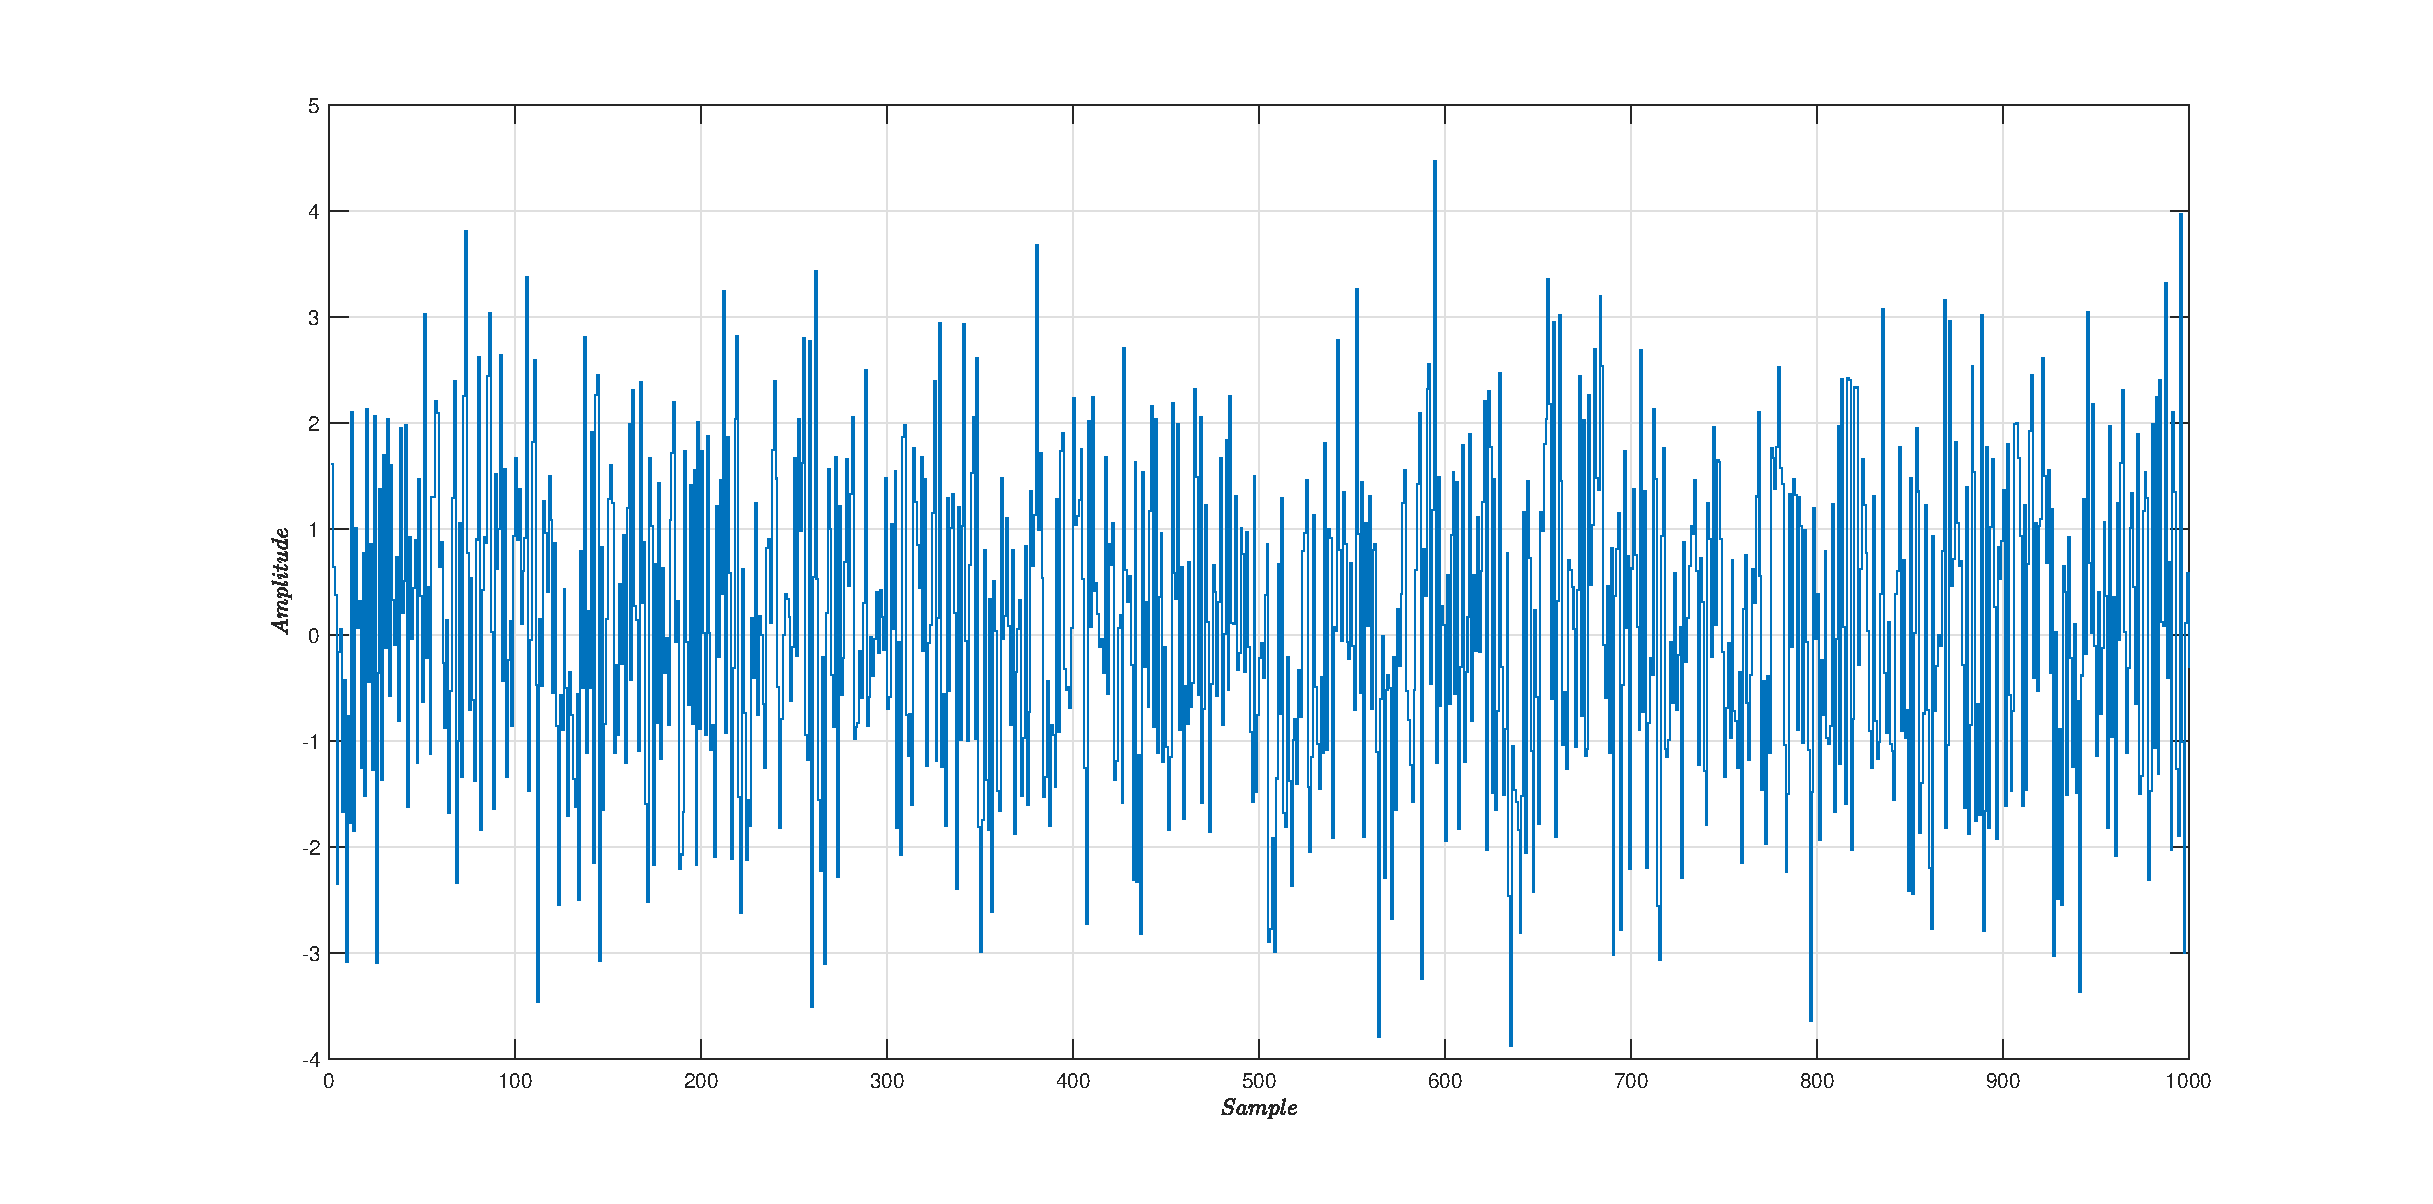
\includegraphics[scale=0.45]{figures/q3f1}
	\caption{Sequence of the Received signal when $\sigma^2 = 1$}
\end{figure}

\begin{figure}[!h]
	\centering
	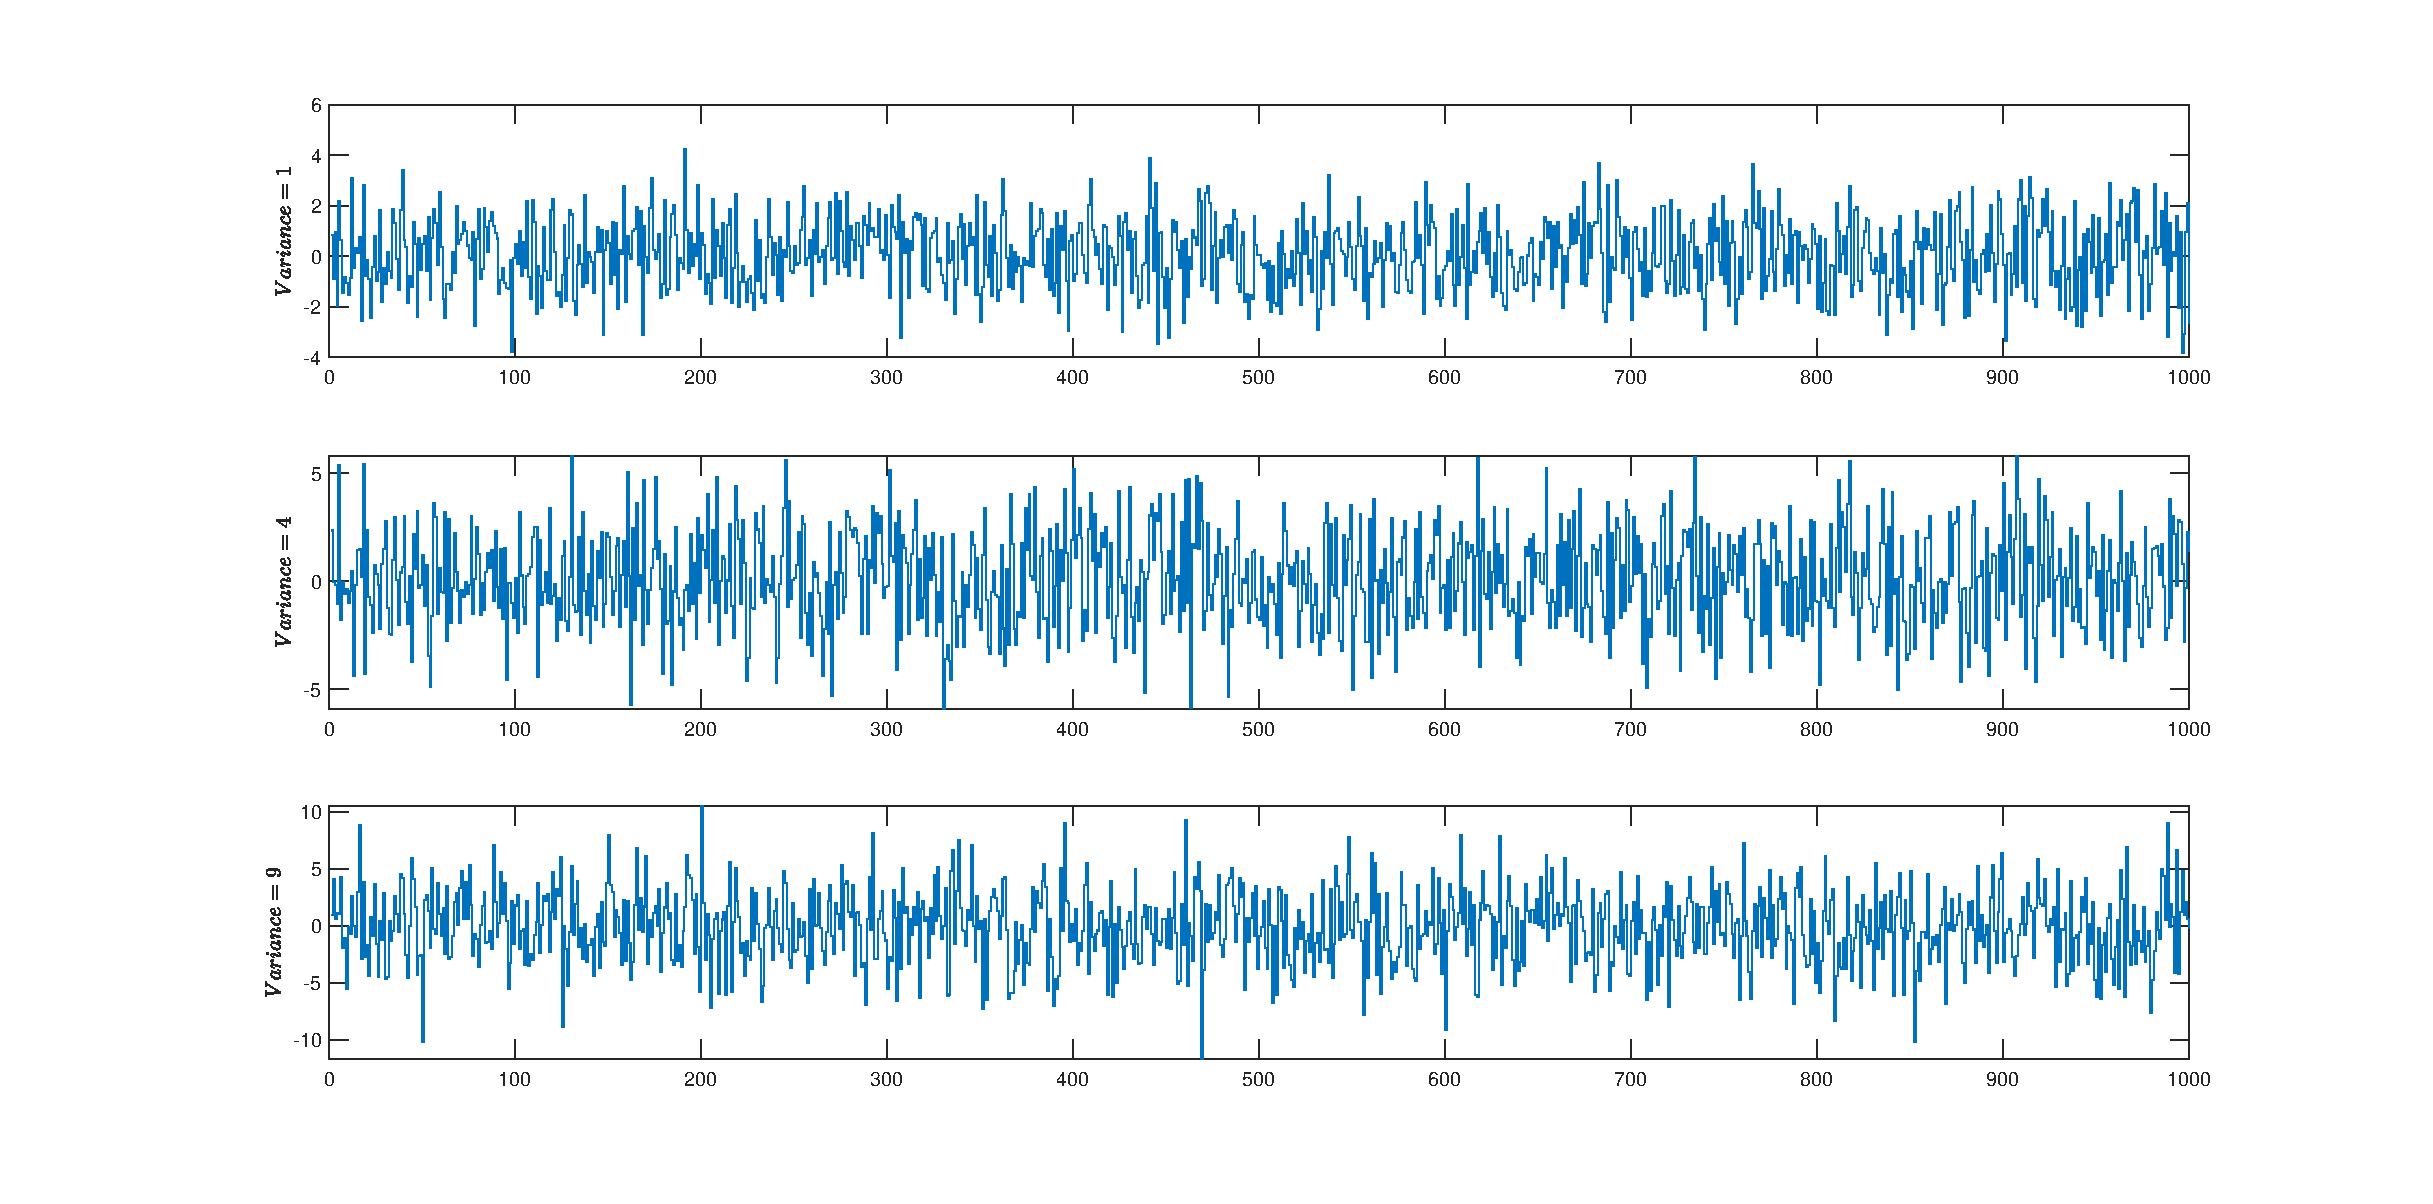
\includegraphics[scale=0.45]{figures/q3f2}
	\caption{Impact of the variance of noise on the Received signal}
\end{figure}

As illustrated in the above figure when the variance of the noise increases the range of the values the received sample can  be in increases (observe the change in the range of Y axis). This essentially increases the bit errors at the receiving end.

\pagebreak
\section{Question 4}
Sketching and comparing the sequence of Y(signal recovered through threshold) with the transmitted signal.
\begin{figure}[!h]
	\centering
	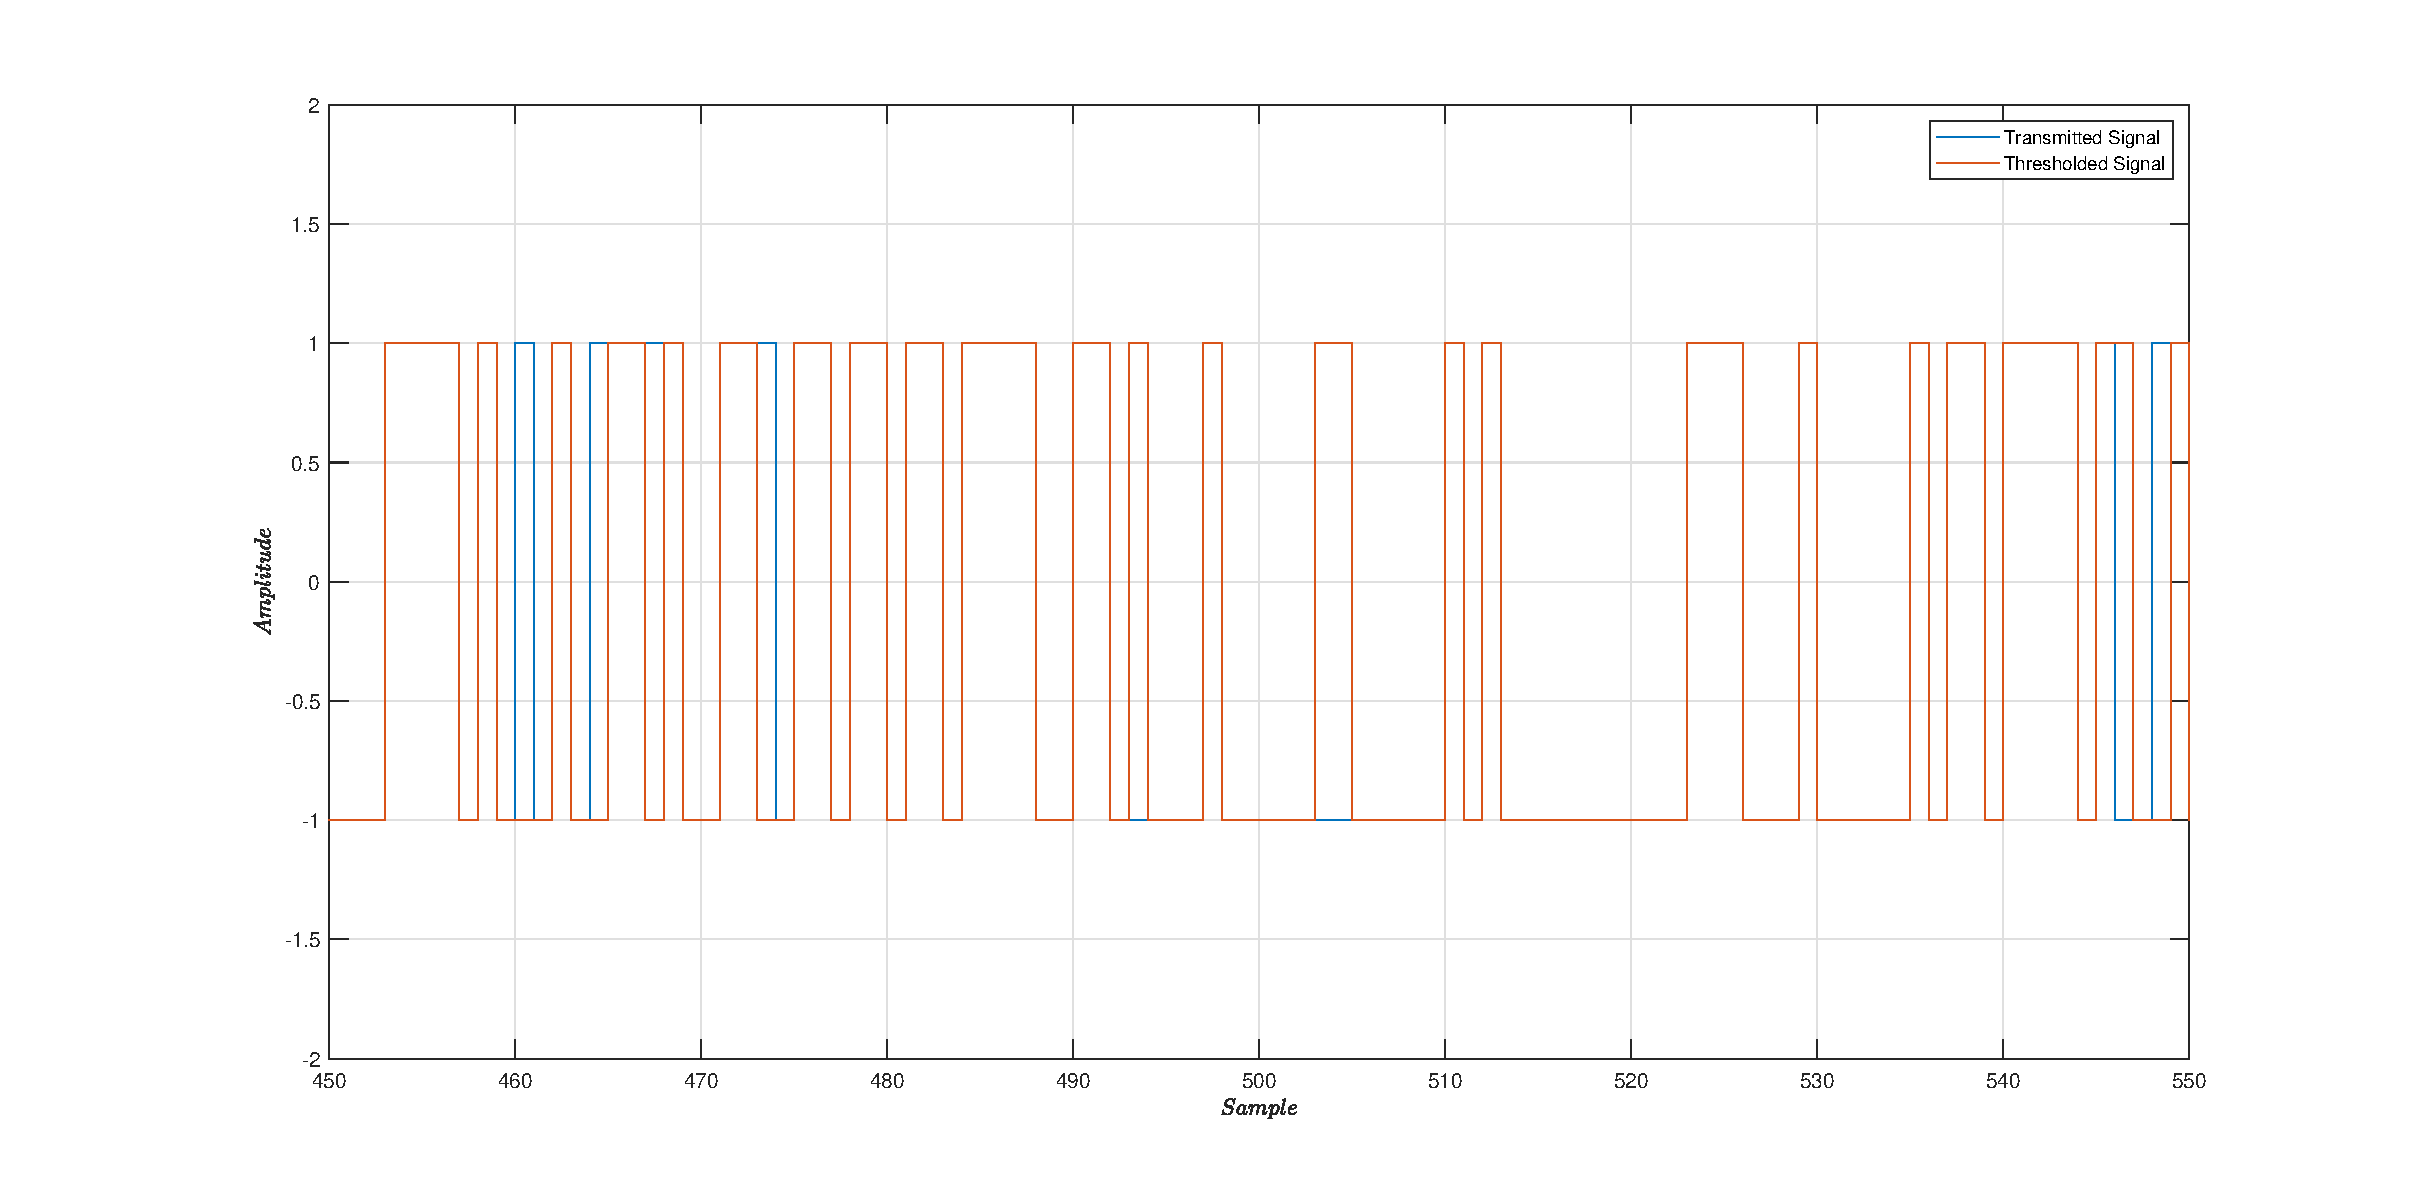
\includegraphics[scale=0.4]{figures/q4f1}
	\caption{Sequence of Y when the number of samples is 1000}
\end{figure}

Most of the transmitted bits have been identified correctly by the receiver after the thresholding(perfectly aligned curves). But some of the bits have been identified incorrectly after the thresholding. Change of signal levels due to the unwanted noise added during the process of transmission is the reason.

\section{Question 5}
Repeating the above steps for a sequence of length L = 100,000.
\begin{figure}[!h]
	\centering
	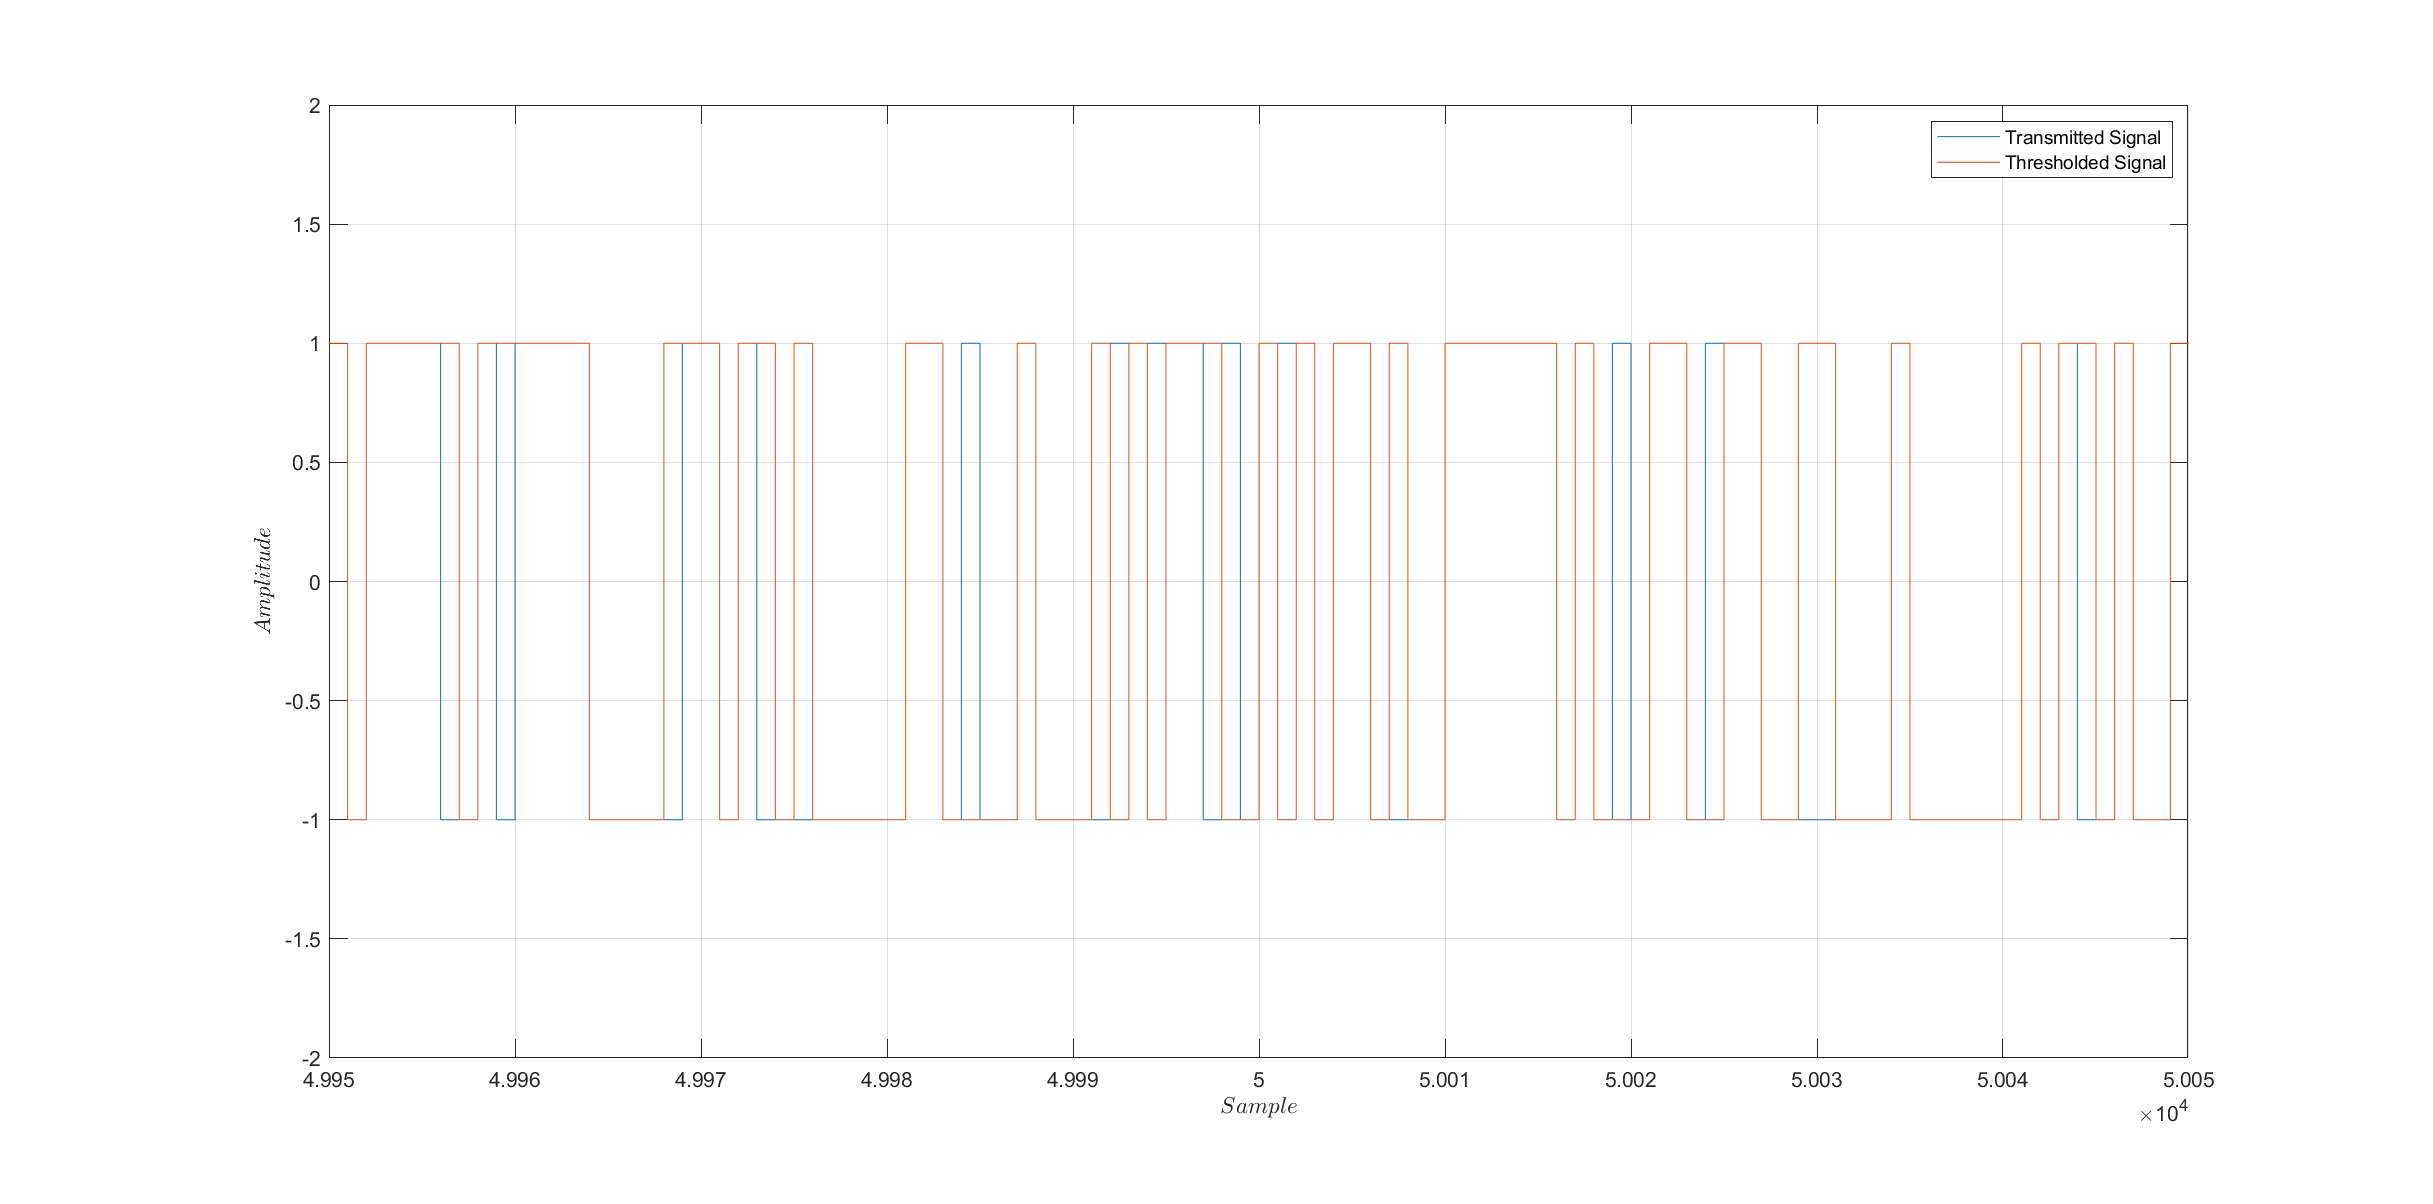
\includegraphics[scale=0.4]{figures/q5f1}
	\caption{Sequence of Y when the number of samples is 100,000}
\end{figure}

The same observations made regarding the previous figure is applicable to this scenario as well. But probability of error has a significant reduction when transmitting a huge number of bits. 

\pagebreak
\subsection{Histogram of the received sequence taking	the no of bins as 10}
\begin{figure}[!h]
	\centering
	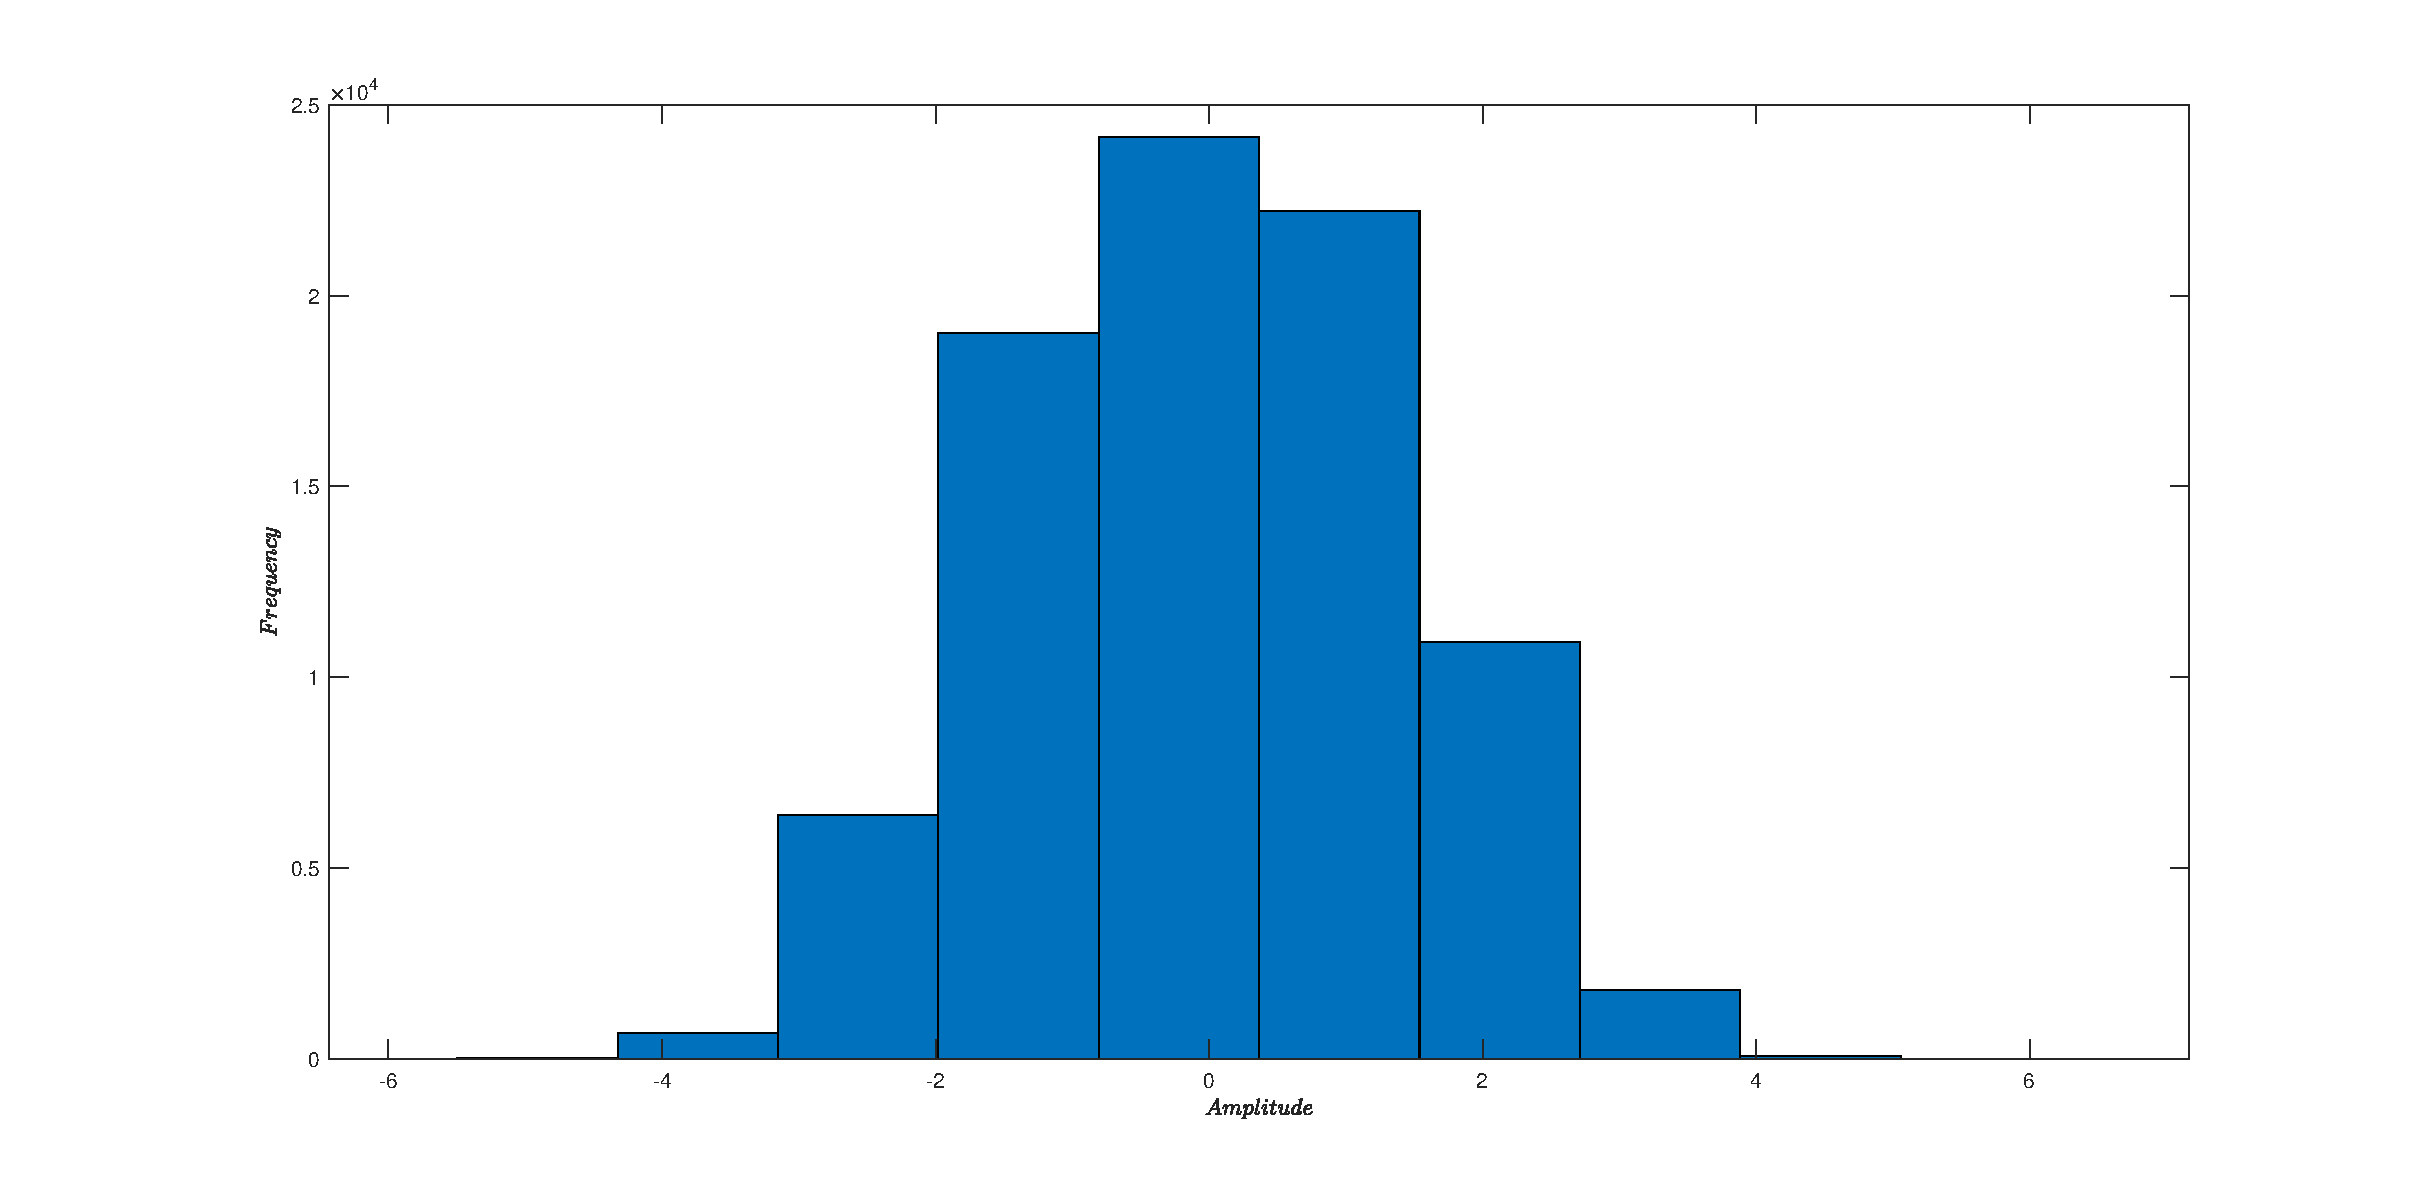
\includegraphics[scale=0.45]{figures/q5f2}
	\caption{Histogram of the received sequence using the user defined function: bins = 10}
\end{figure}

\begin{figure}[!h]
	\centering
	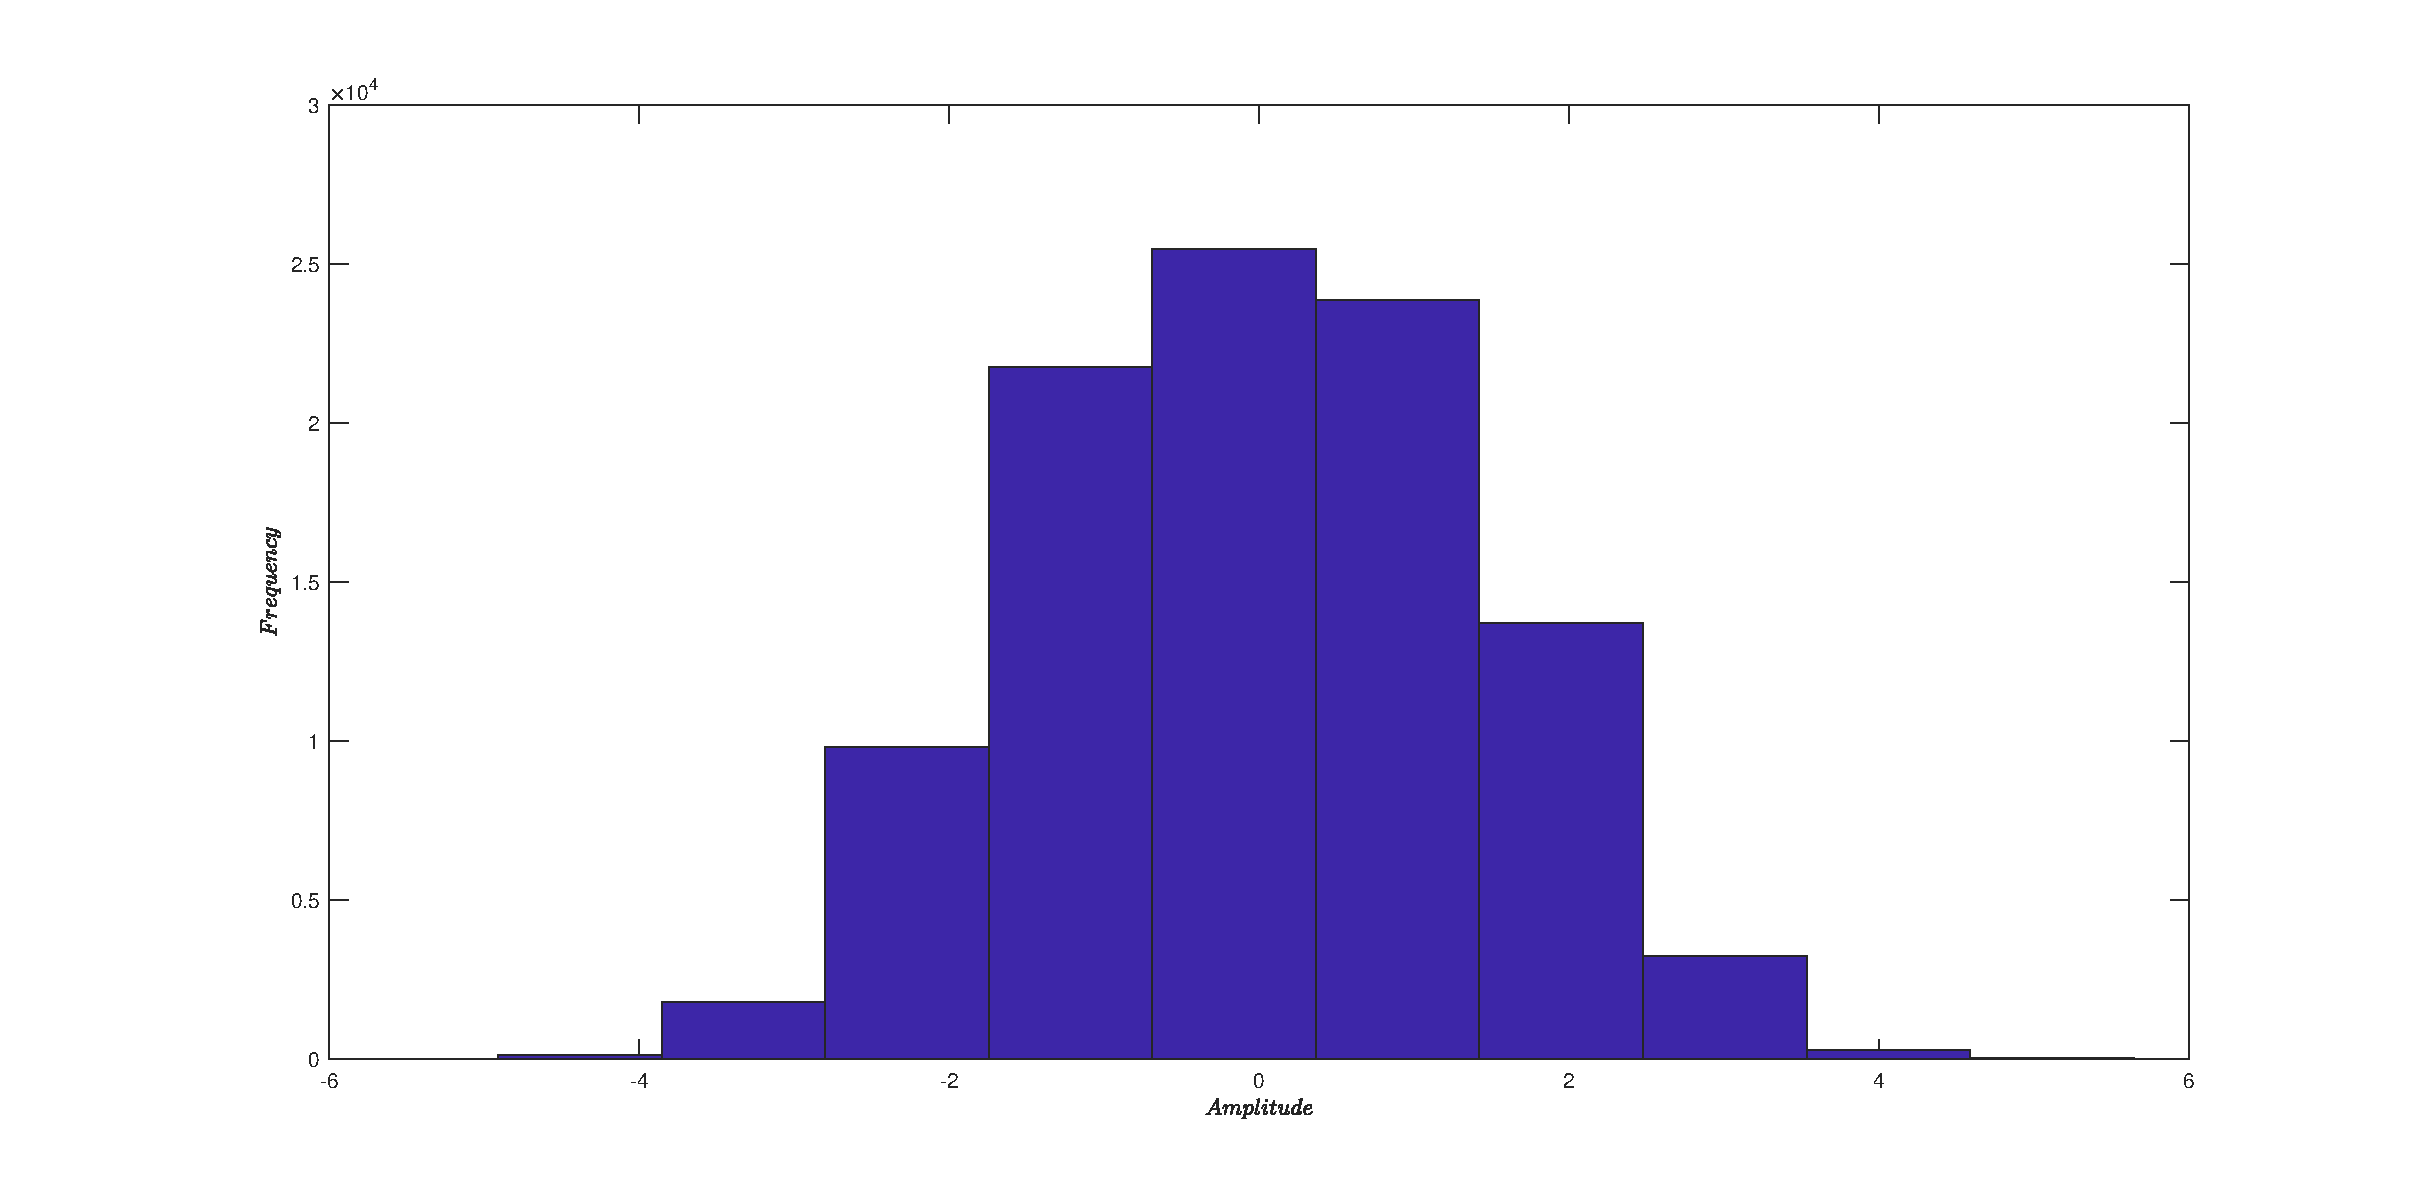
\includegraphics[scale=0.45]{figures/q5f3}
	\caption{Histogram of the received sequence using the MATLAB's built-in {\tt hist()} fucntion: bins = 10}
\end{figure}

\textbf{Comparison} : Histograms generated using the custom user defined function and the built-in function are almost the same. The reason for the difference in frequencies can be identified as the range differences of bins considered in the two algorithms. Code of the user defined fucntion can be found at the end of the Appendix.

\pagebreak
\subsection{Impact when the number of bins is changed from 10 to 100}

\begin{figure}[!h]
	\centering
	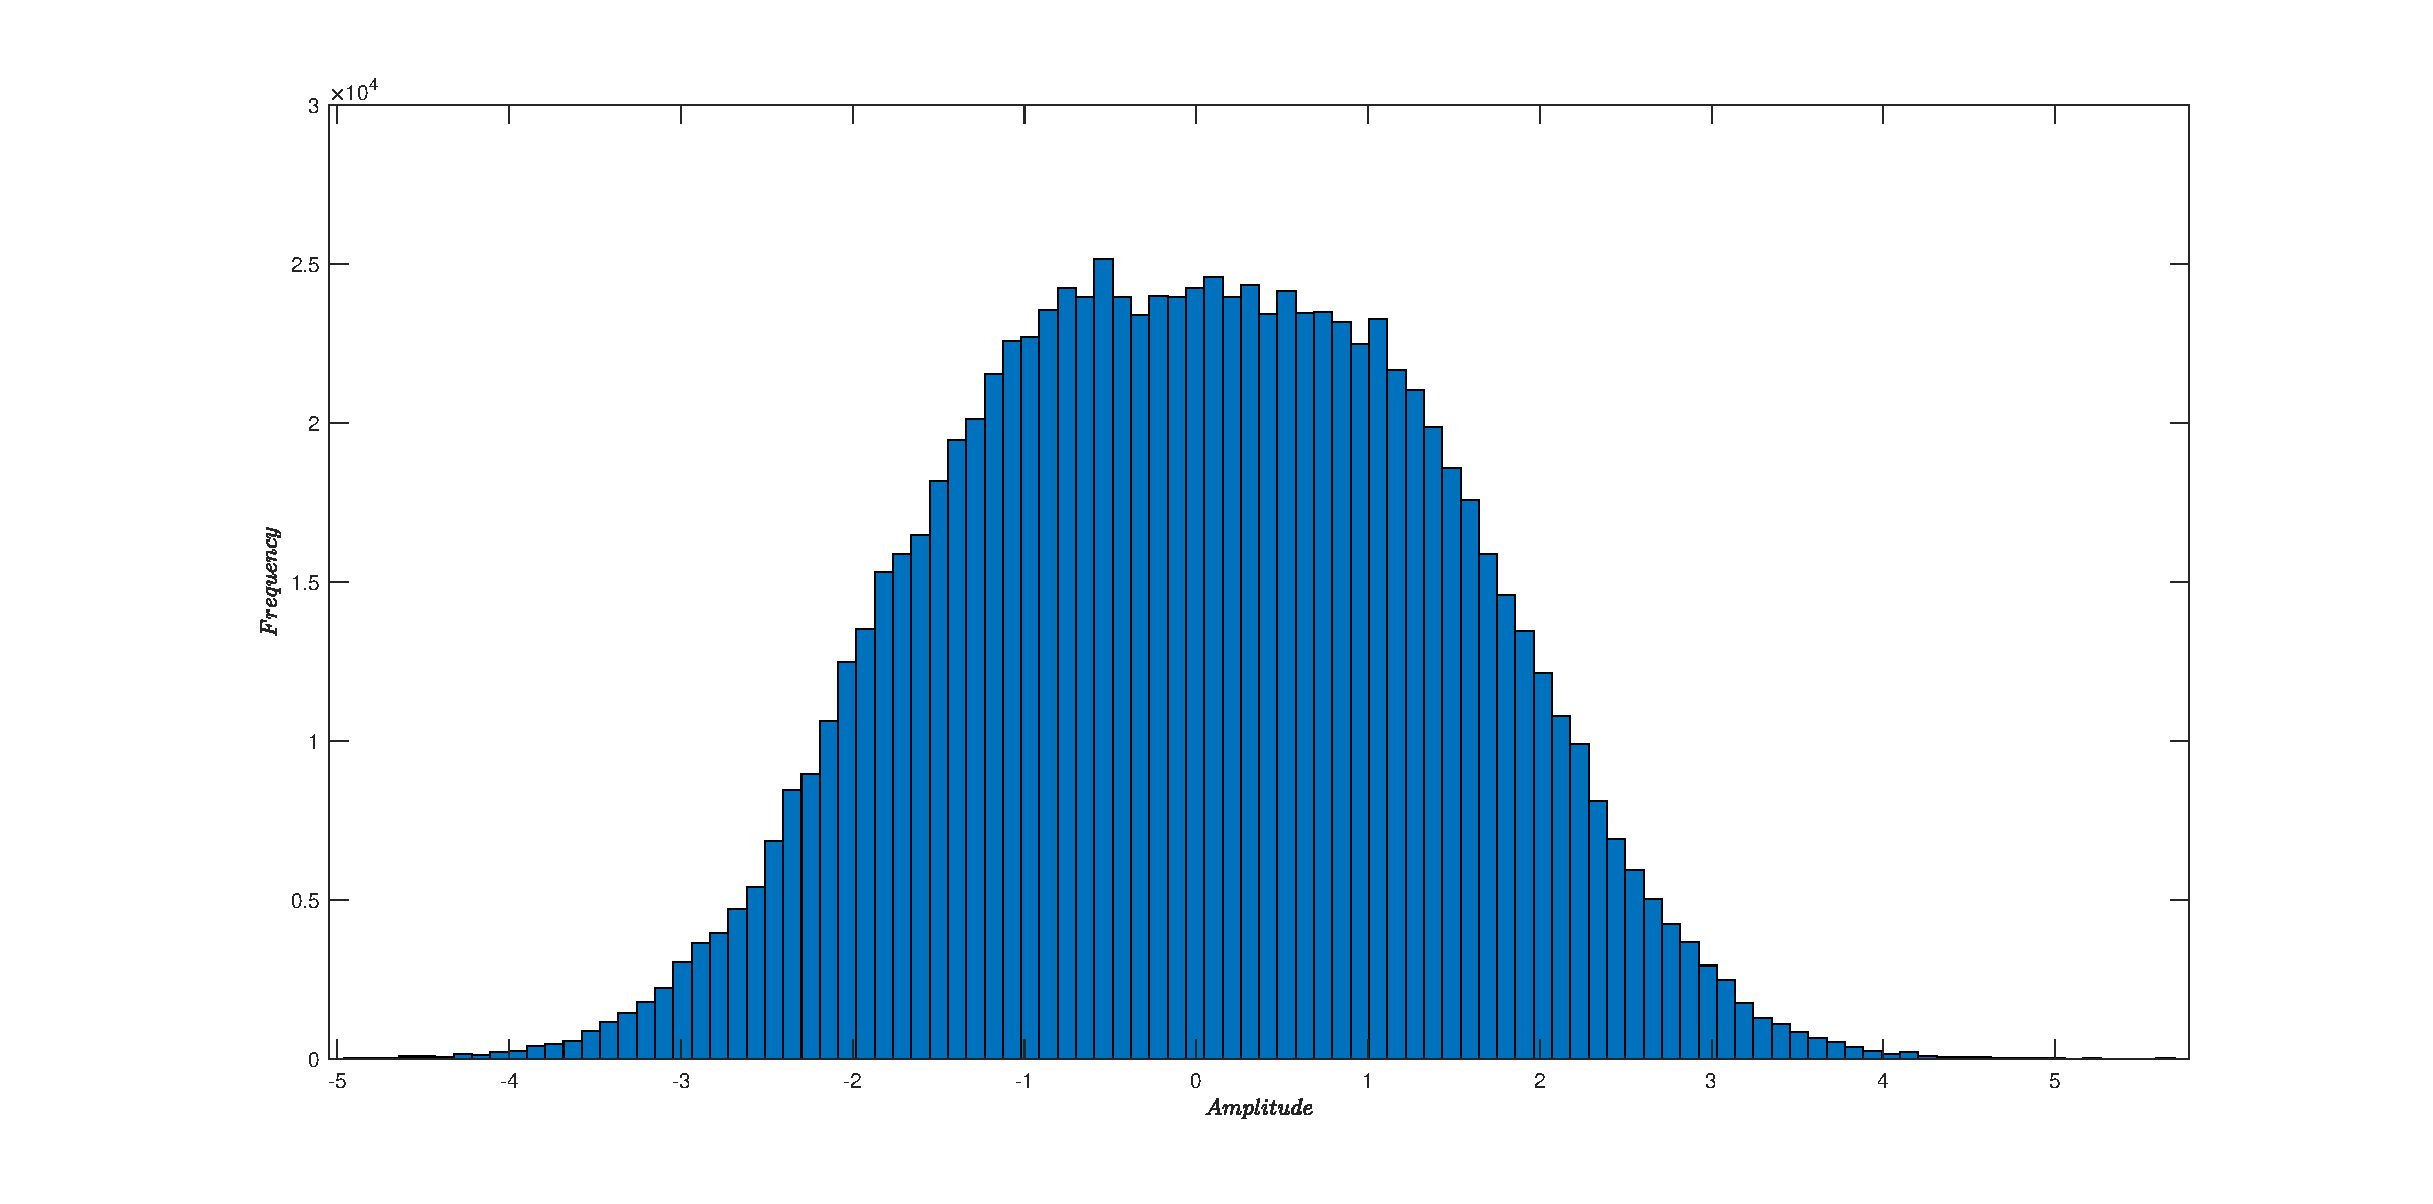
\includegraphics[scale=0.45]{figures/q5f4}
	\caption{Histogram of the received sequence using the user defined function: bins =100}
\end{figure}

\begin{figure}[!h]
	\centering
	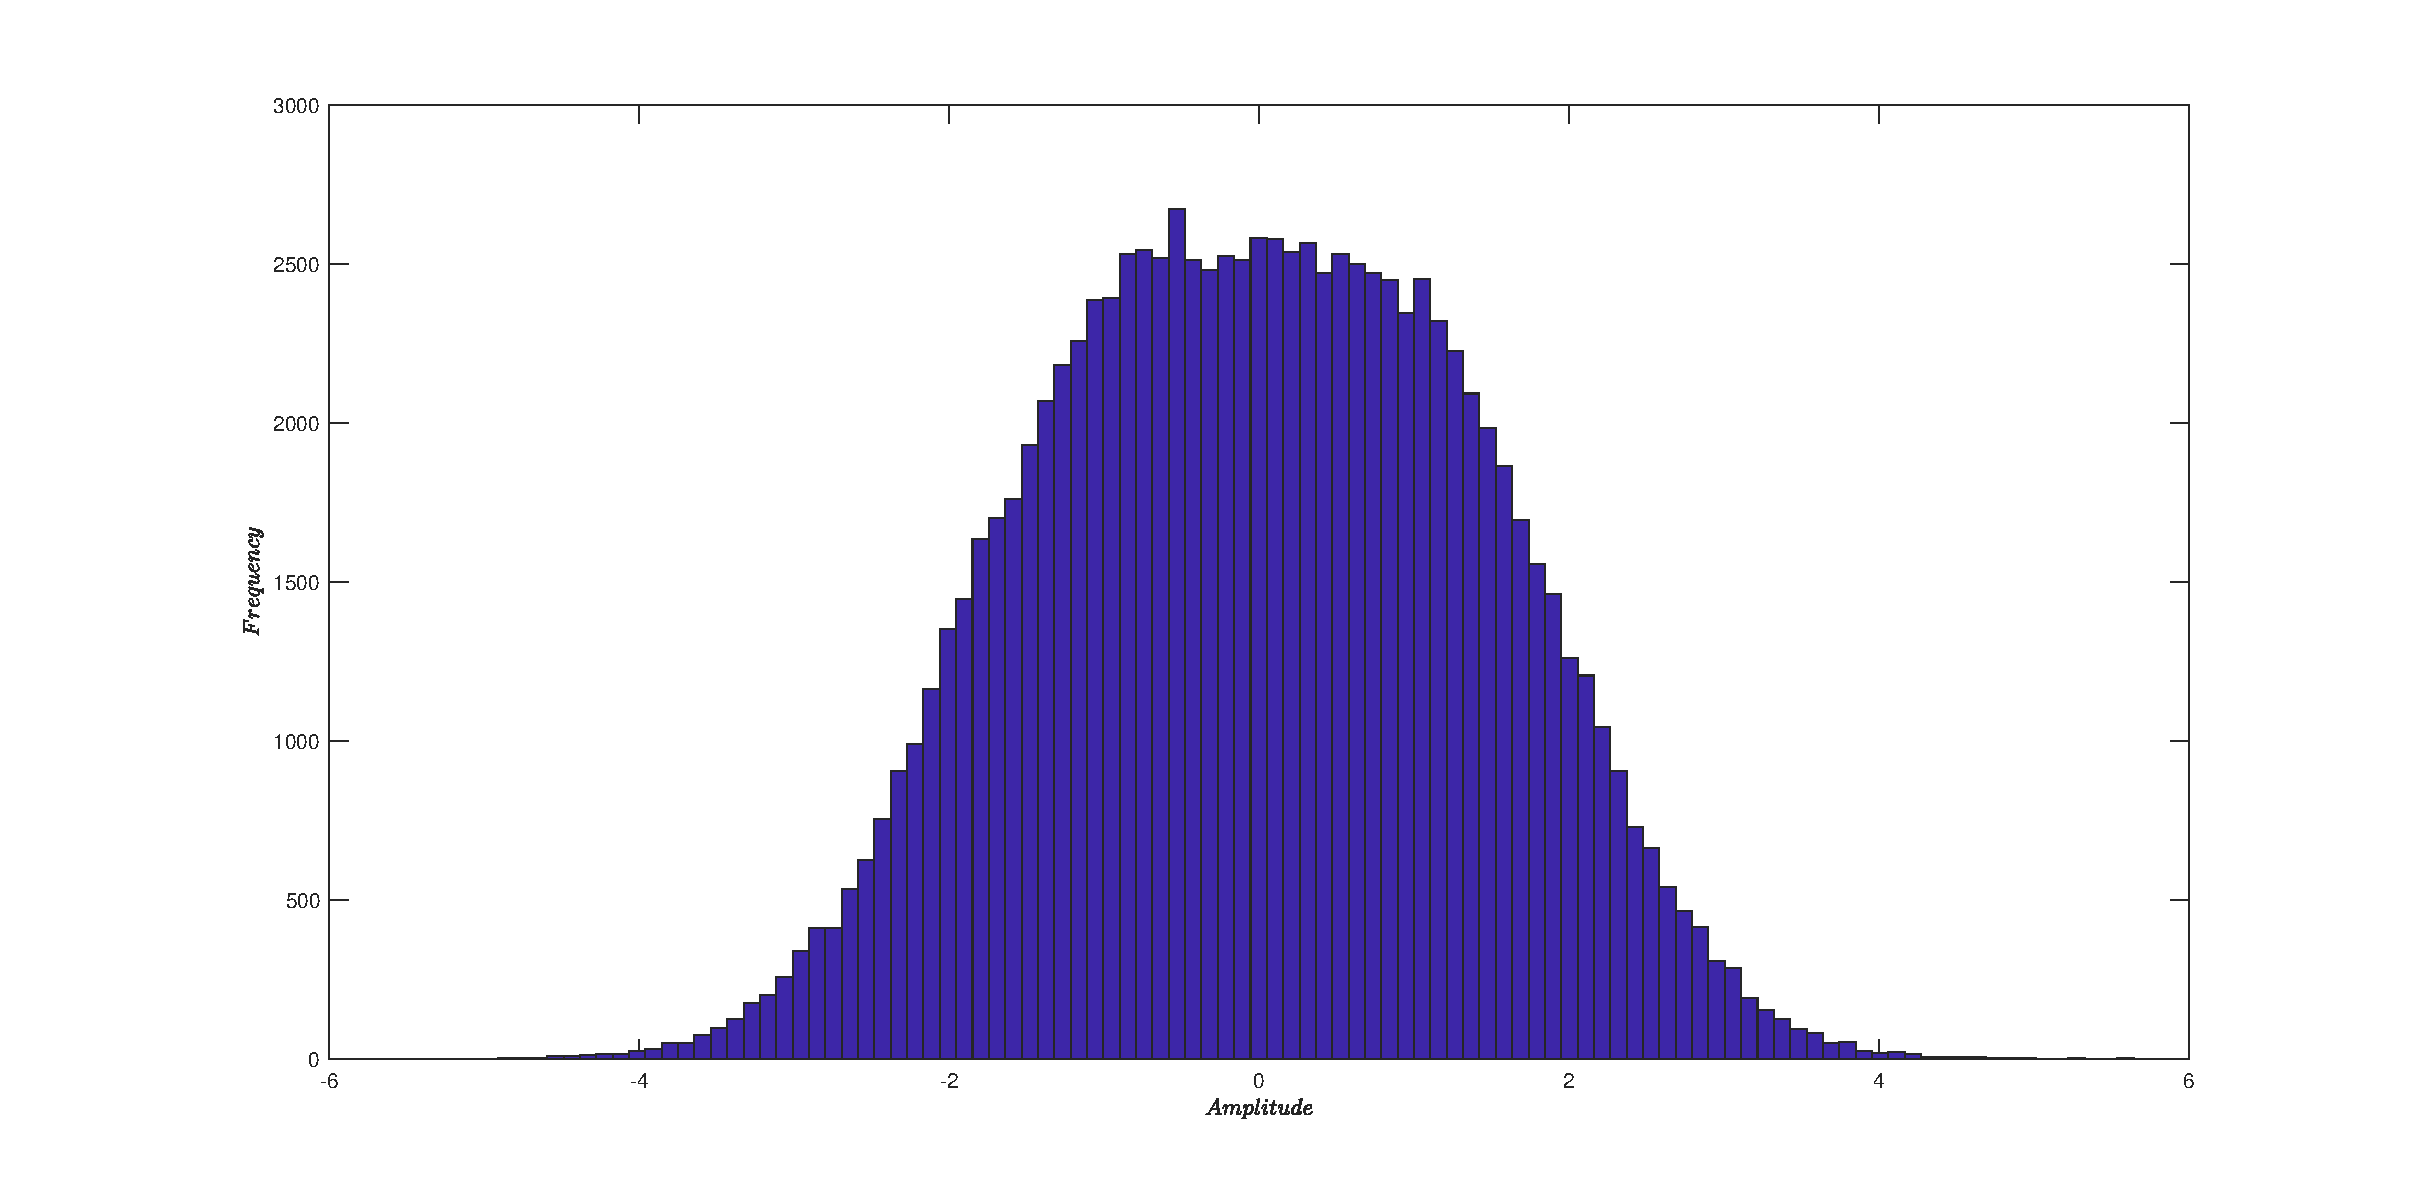
\includegraphics[scale=0.45]{figures/q5f5}
	\caption{Histogram of the received sequence using the MATLAB's built-in {\tt hist()} fucntion: bins = 100}
\end{figure}
\textbf{Impact}: When the number of bins is changed from 10 to 100, shape of the normal distribution becomes clearly visible and differences between two histograms become negligible as the ranges of the bins become more similar.

\pagebreak
\subsection{Conditional PDFs when number of bins = 100 and A = 1}

Dependent axis represents the normalized frequencies calculated as follows. And therefore following figures illustrates the approximation for the required Probability Density Functions.
\[
Normalized ~Freq = \frac{Frequency}{Total~Number~of~Samples \times Width~of~a~Bin}
\] 

\begin{figure}[!h]
	\centering
	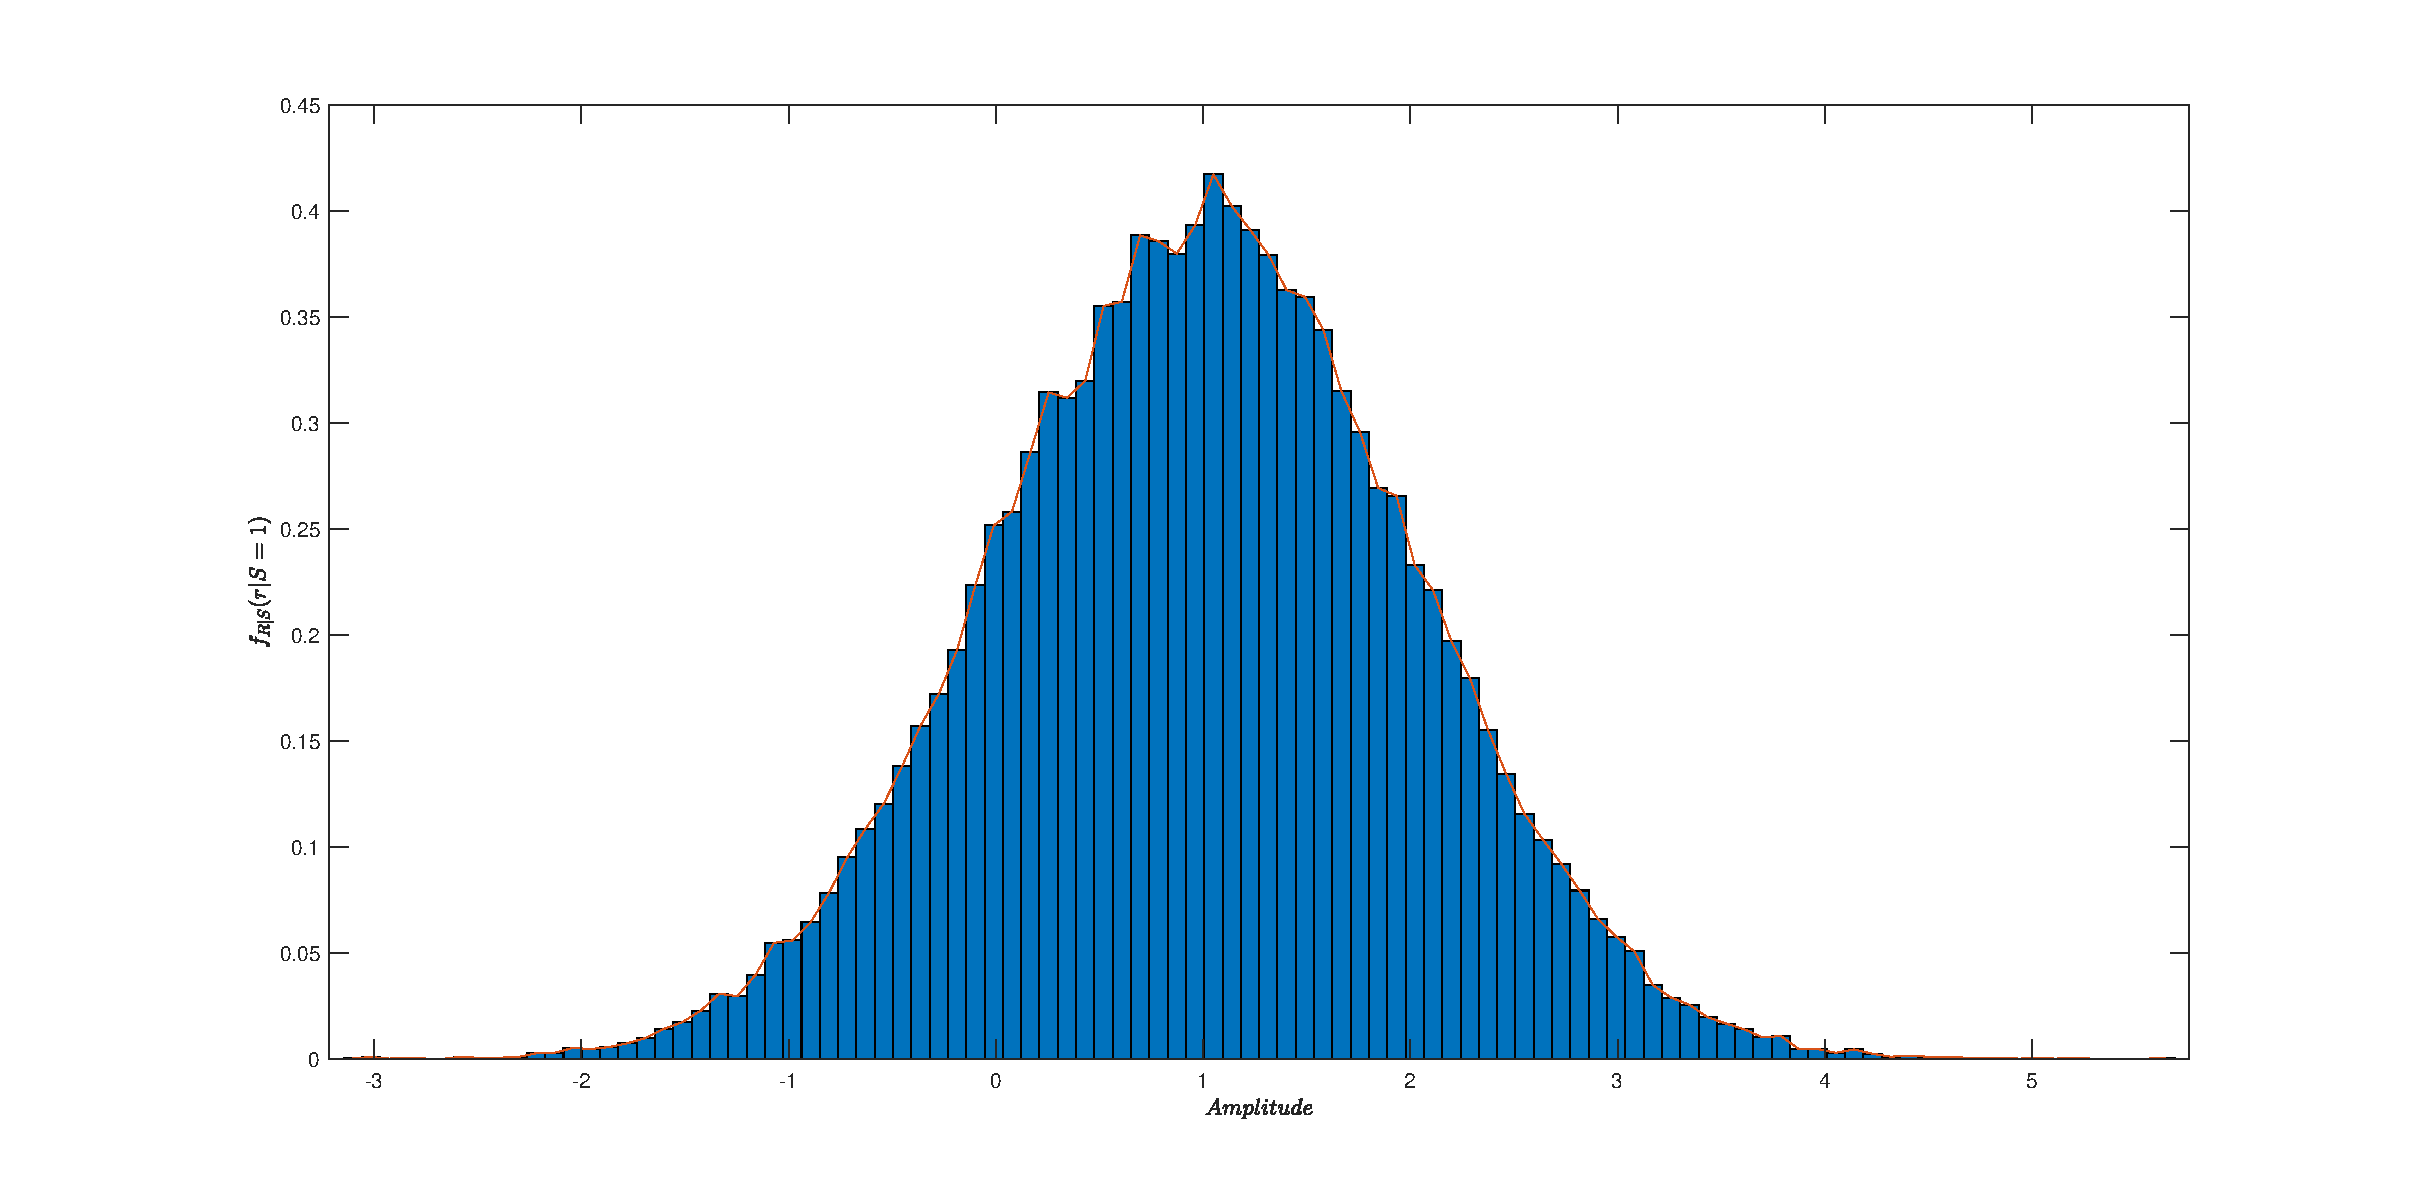
\includegraphics[scale=0.45]{figures/q5f6}
	\caption{$f_{R|S}(r|S=A)$ when A = 1: Mean $\approx$ 1}
\end{figure}

\begin{figure}[!h]
	\centering
	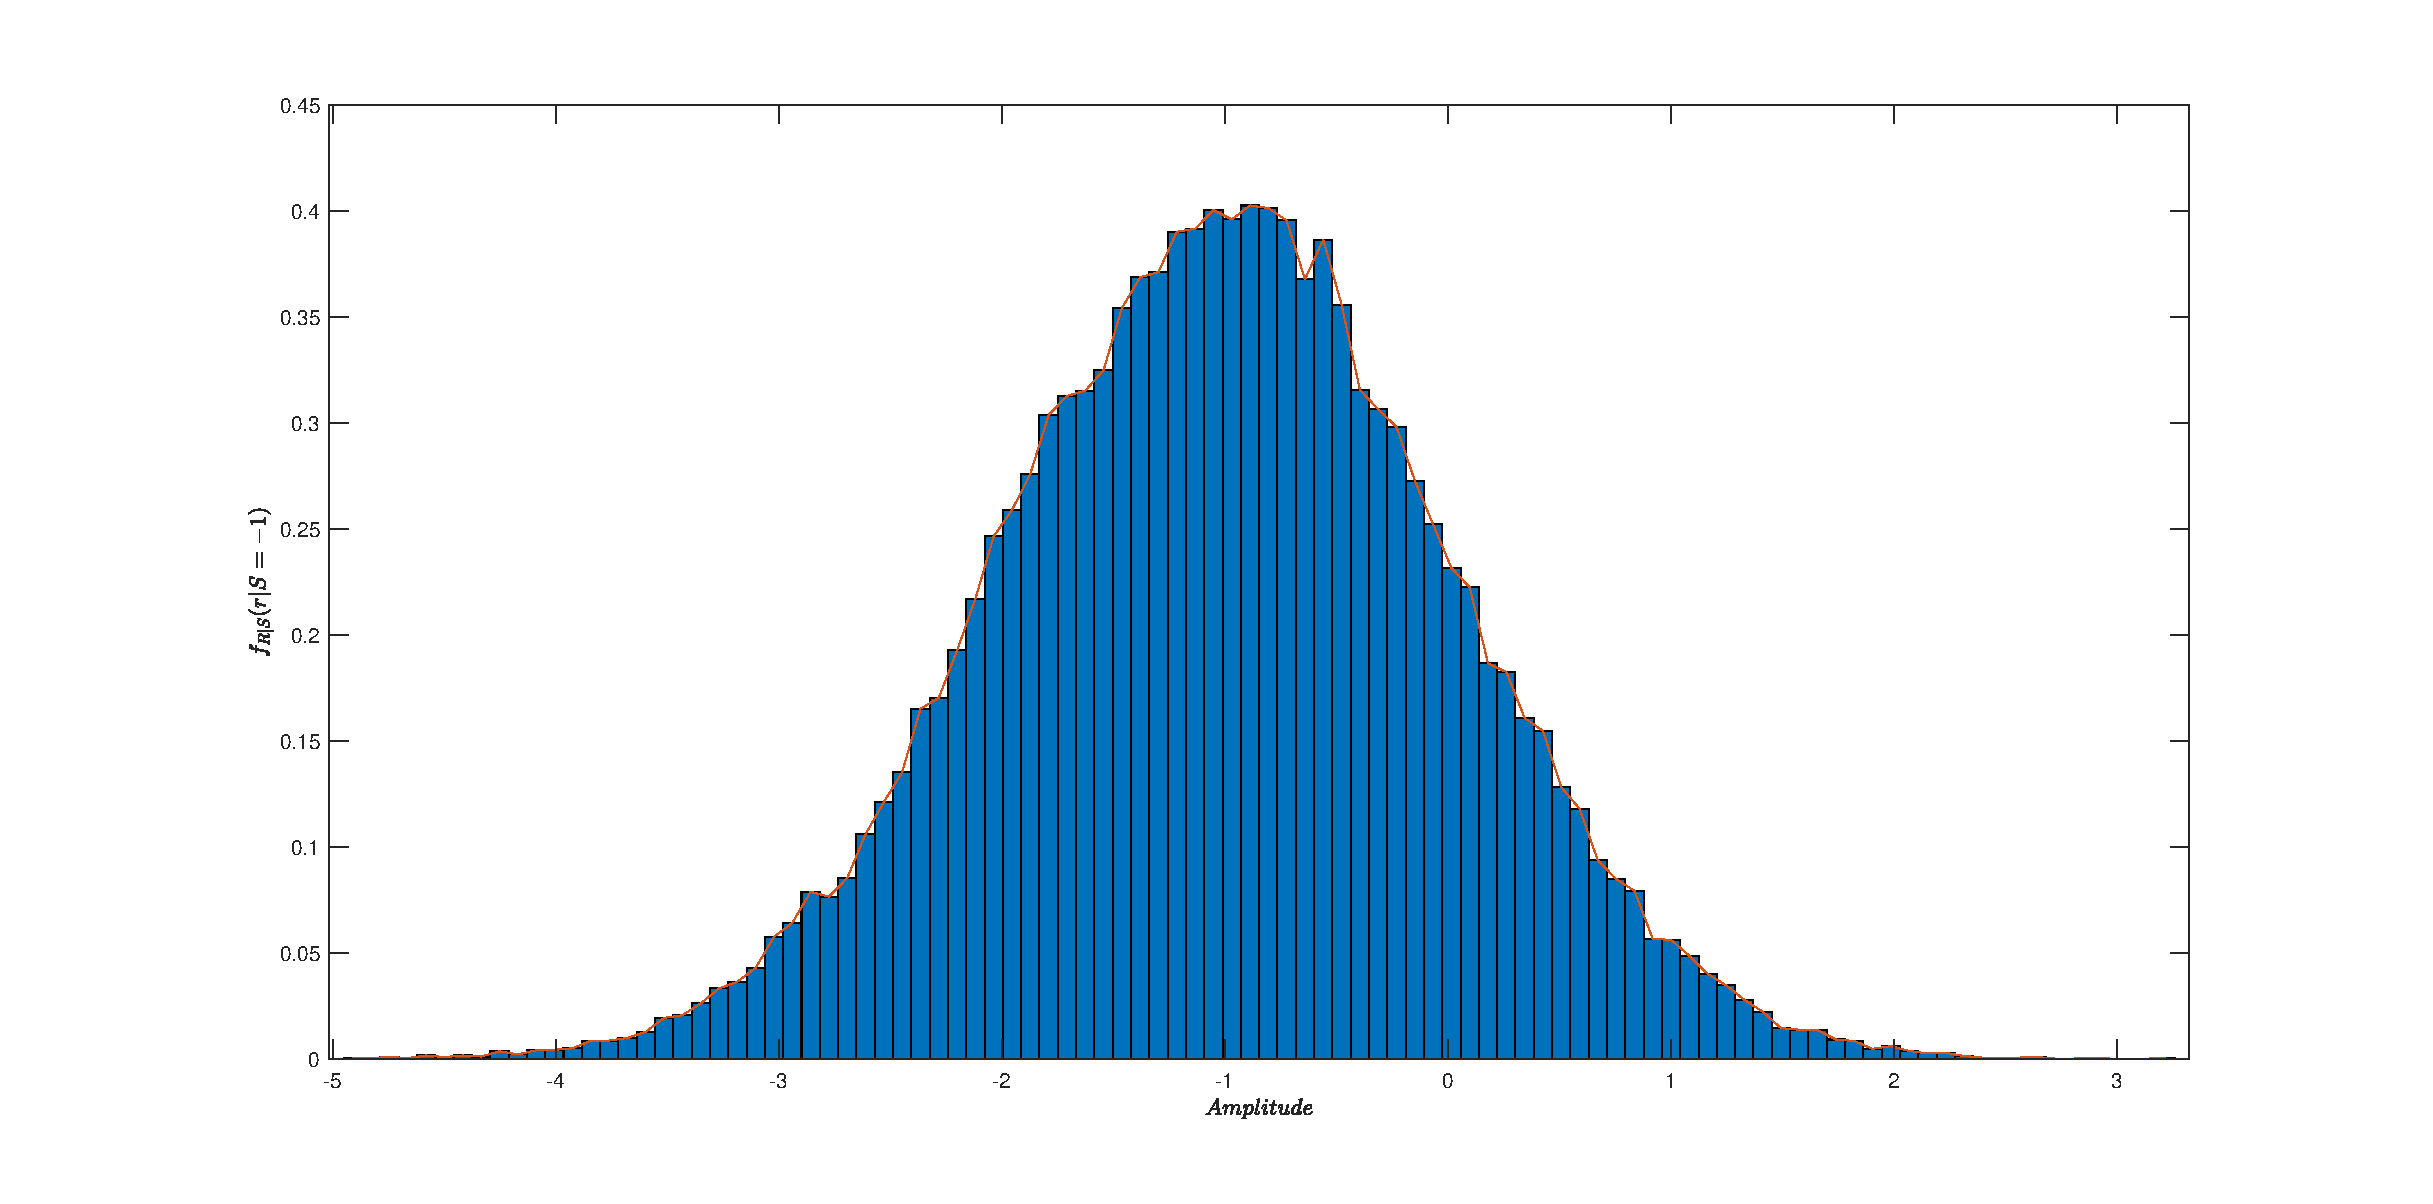
\includegraphics[scale=0.45]{figures/q5f7}
	\caption{$f_{R|S}(r|S= -A)$ when A =1: Mean $\approx$ -1}
\end{figure}

Observe that when the distribution is conditioned on S, the mean of the distribution shifts along the amplitude axis towards the S.

\pagebreak
\subsection{Impact of A on the Conditional PDFs}

As illustrated in the following figures, when the distribution is conditioned on S =A , the mean of the distribution shifts along the amplitude axis towards the S = A.  But the variance of the distribution remains the same as it is only affected by the AWGN.

\begin{figure}[!h]
	\centering
	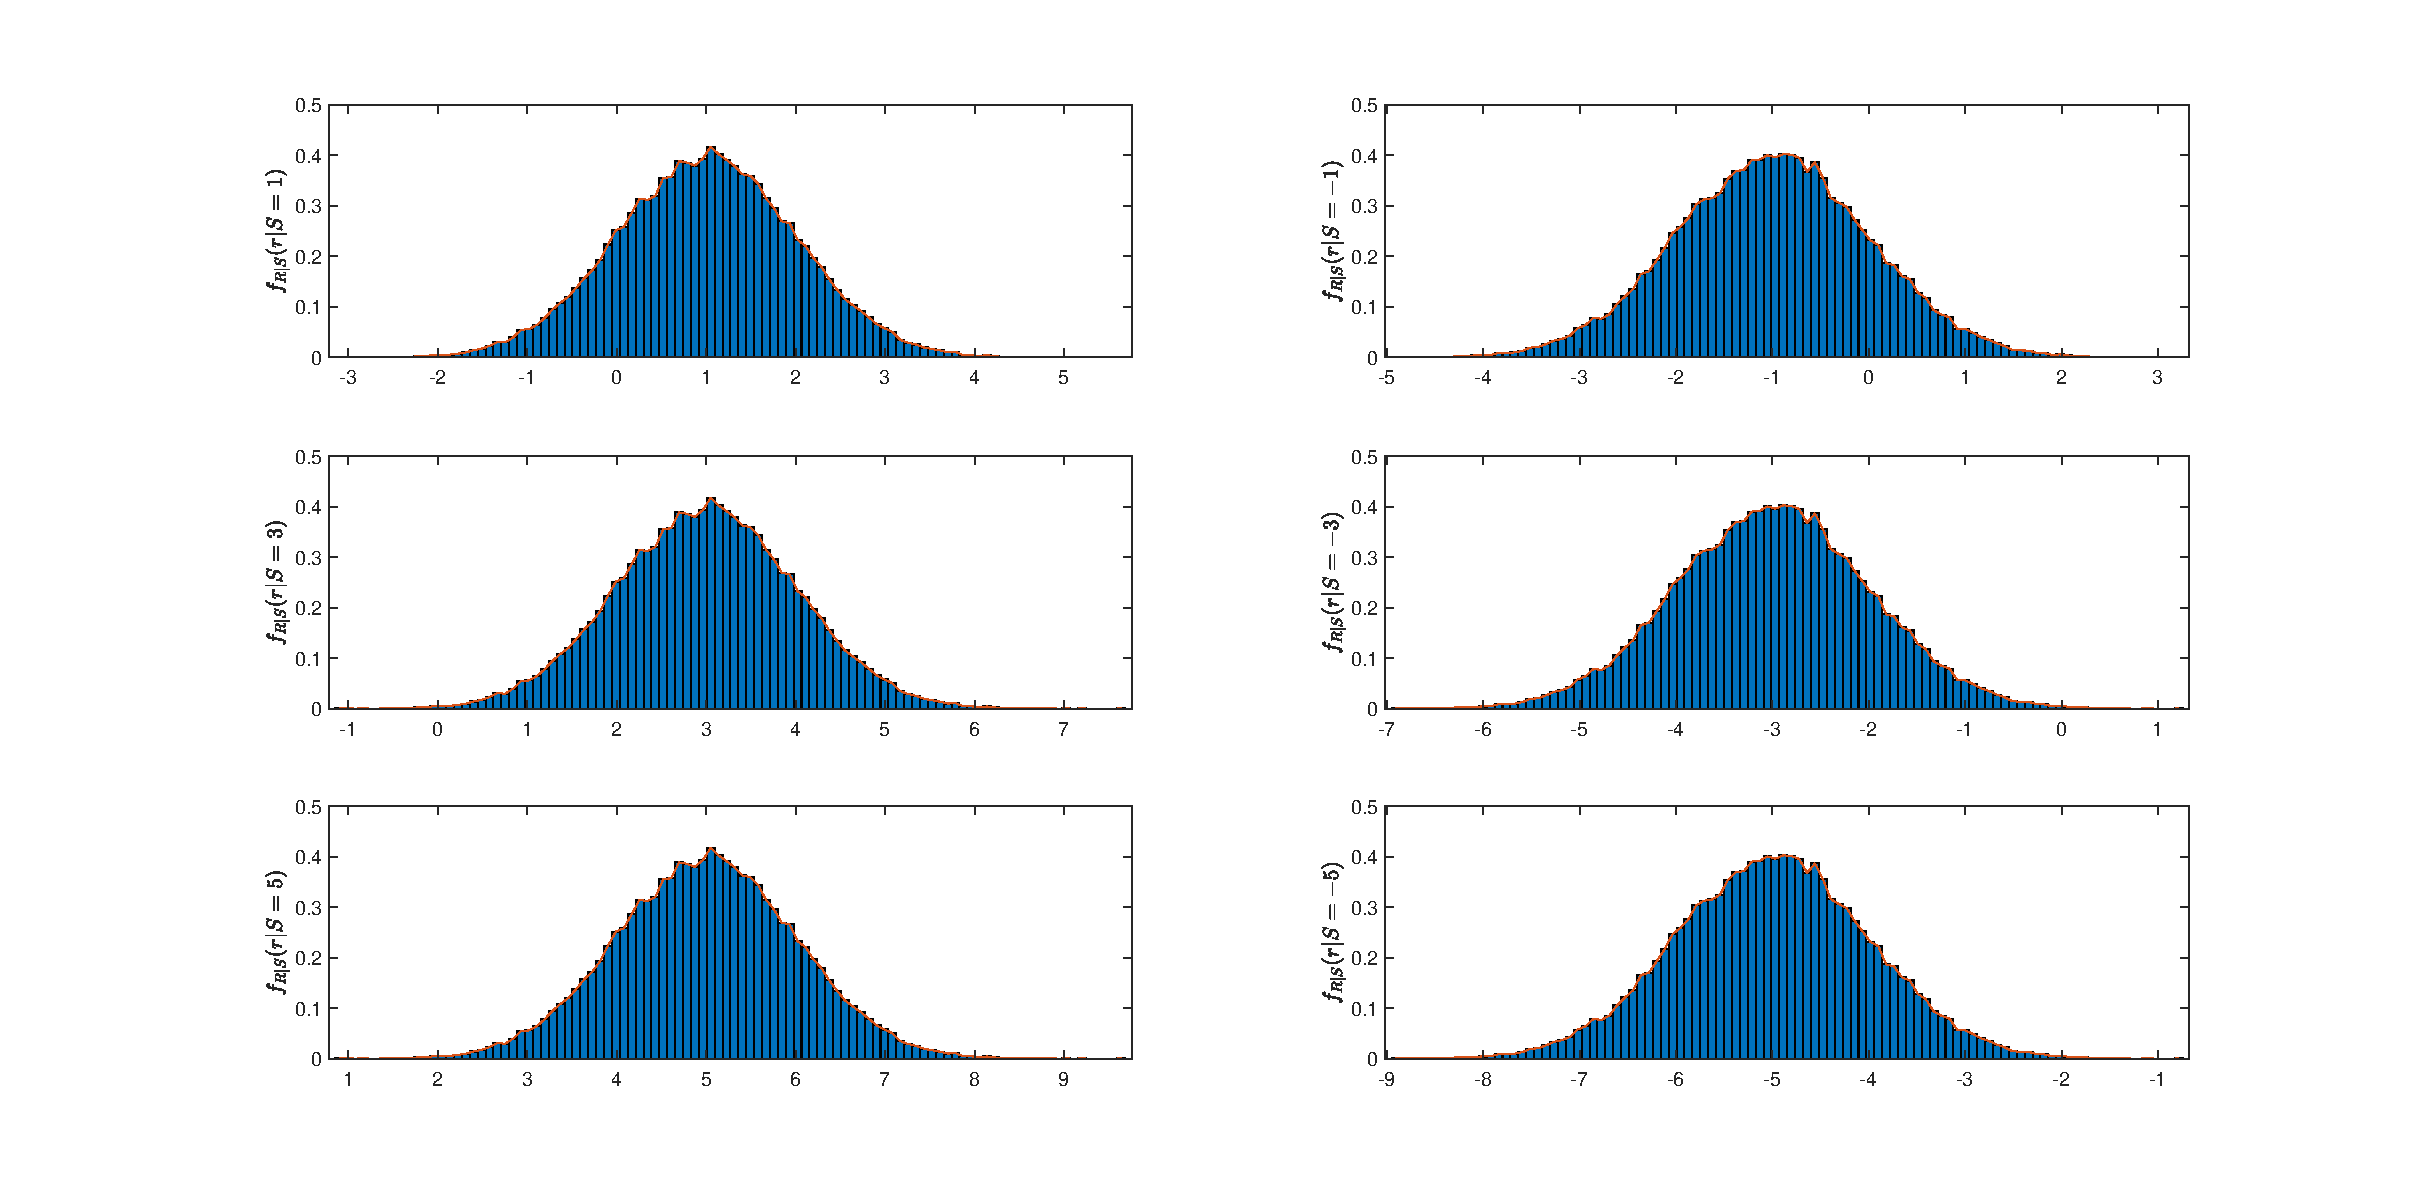
\includegraphics[scale=0.45]{figures/q5f8}
	\caption{Impact of A on the Conditional PDFs}
\end{figure}

\subsection{Expected Values of the distributions when A = 1}

The expected value of a continuous Random variable $X$ which has a PDF of $f_X(x)$ is given as,
\[
E[X] = \int_{-\infty}^{+\infty} x.f_X(x) ~dx
\]
The same formula can be redefined for discrete case as follows where $\Delta x$ represents the width of a bin which is equal in our cases.
\[
E[X] = \sum_{i = 1}^{N} x_i.P(x_i).\Delta x
\]

Therefore the requires expected values can be easily found using the {\tt Expected(x, px, bin\_width)} function defined in the appendix. The required parameters of that function can be found using the {\tt myHistogram(valueArray,numberOfBins, Normalized)} function. \\

\begin{tabular}[!h]{l c r}
	Expected value $E[R]$& = & -0.00073493\\
Expected value $E[R|S=A]$ &=& 1.0004\\
Expected value $E[R|S=-A]$& =& -1.0011\\

\end{tabular}

\pagebreak
\subsection{Marginal PDF of R $f_R(r)$}
Dependent axis represents the normalized frequencies calculated as follows as mentioned previously. Therefore, the following figure illustrates the approximation for the required Marginal Probability Density Functions of the continuous Random Variable R.
\[
Normalized ~Freq = \frac{Frequency}{Total~Number~of~Samples \times Width~of~a~Bin}
\] 

Expected value of the Random Variable  ($E[R]$ = -0.00073493) reaches zero as the probabilities Pr(D = 0) = Pr(D = 1) = 1/2 are equal.

\begin{figure}[!h]
	\centering
	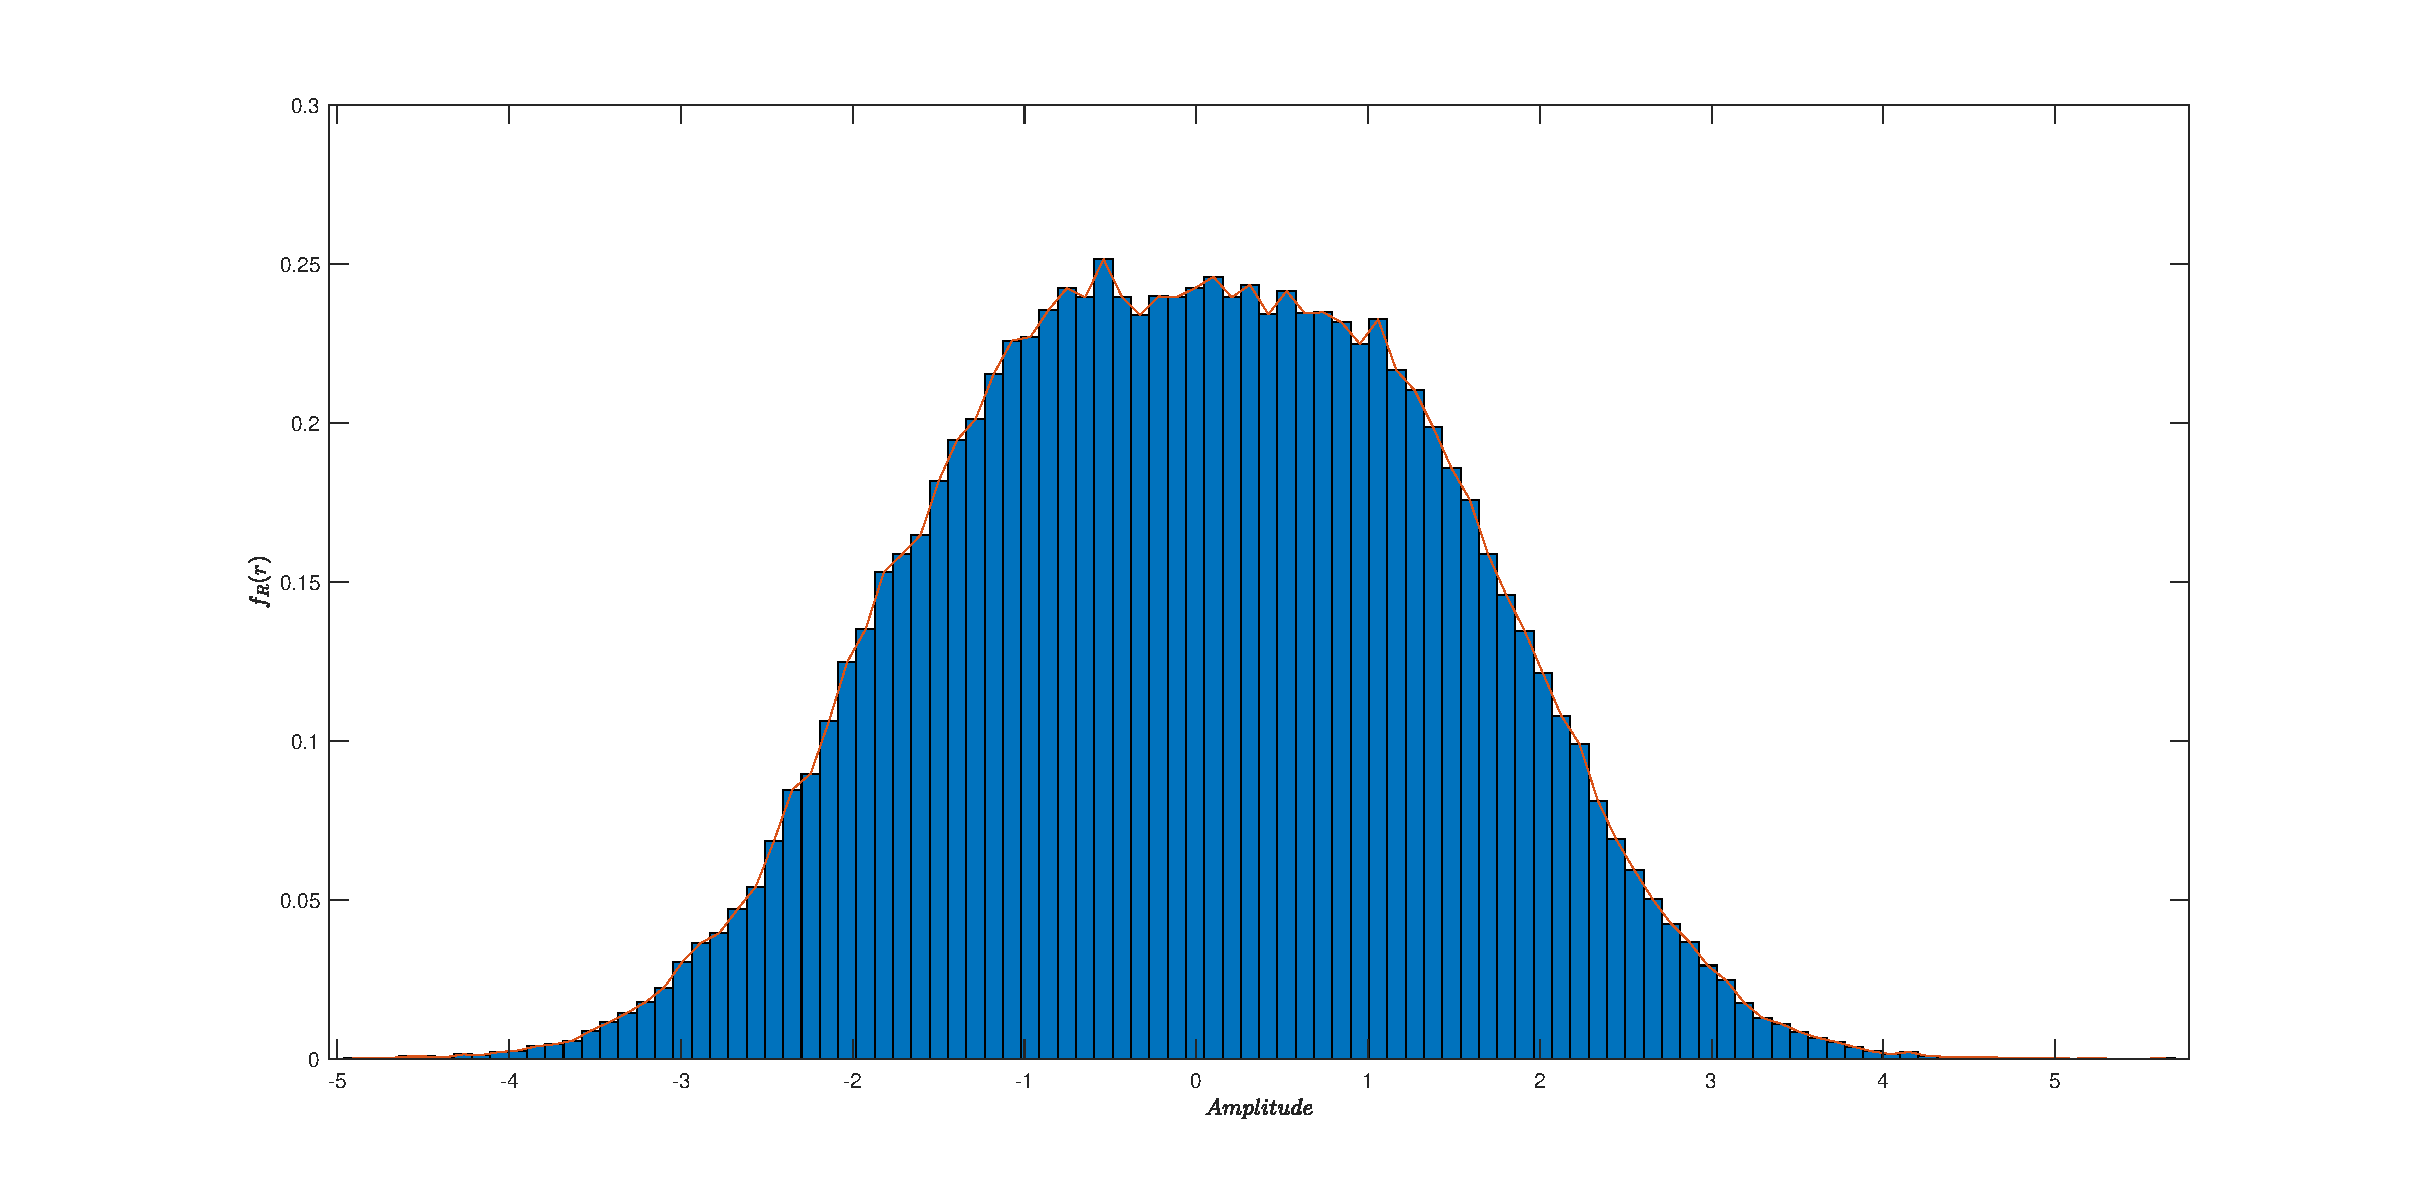
\includegraphics[scale=0.45]{figures/q5f9}
	\caption{Marginal PDF of R $f_R(r)$}
\end{figure}


\pagebreak
\section{Question 6: Effect of Interference}

Interference does nothing other than increasing the variance of the  distribution. When comparing the following figures with the figures of the previous section it is clearly visible. As the variance increases, to keep the area under the graph  a constant, the peak of the graph lowers. Therefore following two observations can be made when additional interference is added to the transmitted signal.
\begin{itemize}
	\item Variance of the distribution increases. Which eventually increases the probability of error.
	\item Peak value of the distribution decreases to keep the area under the curve constant.
\end{itemize}

These observations are common to all the figures and subsections of this section.

\subsection{Conditional PDFs when number of bins = 100, A = 1 and under additional interference}

\begin{figure}[!h]
	\centering
	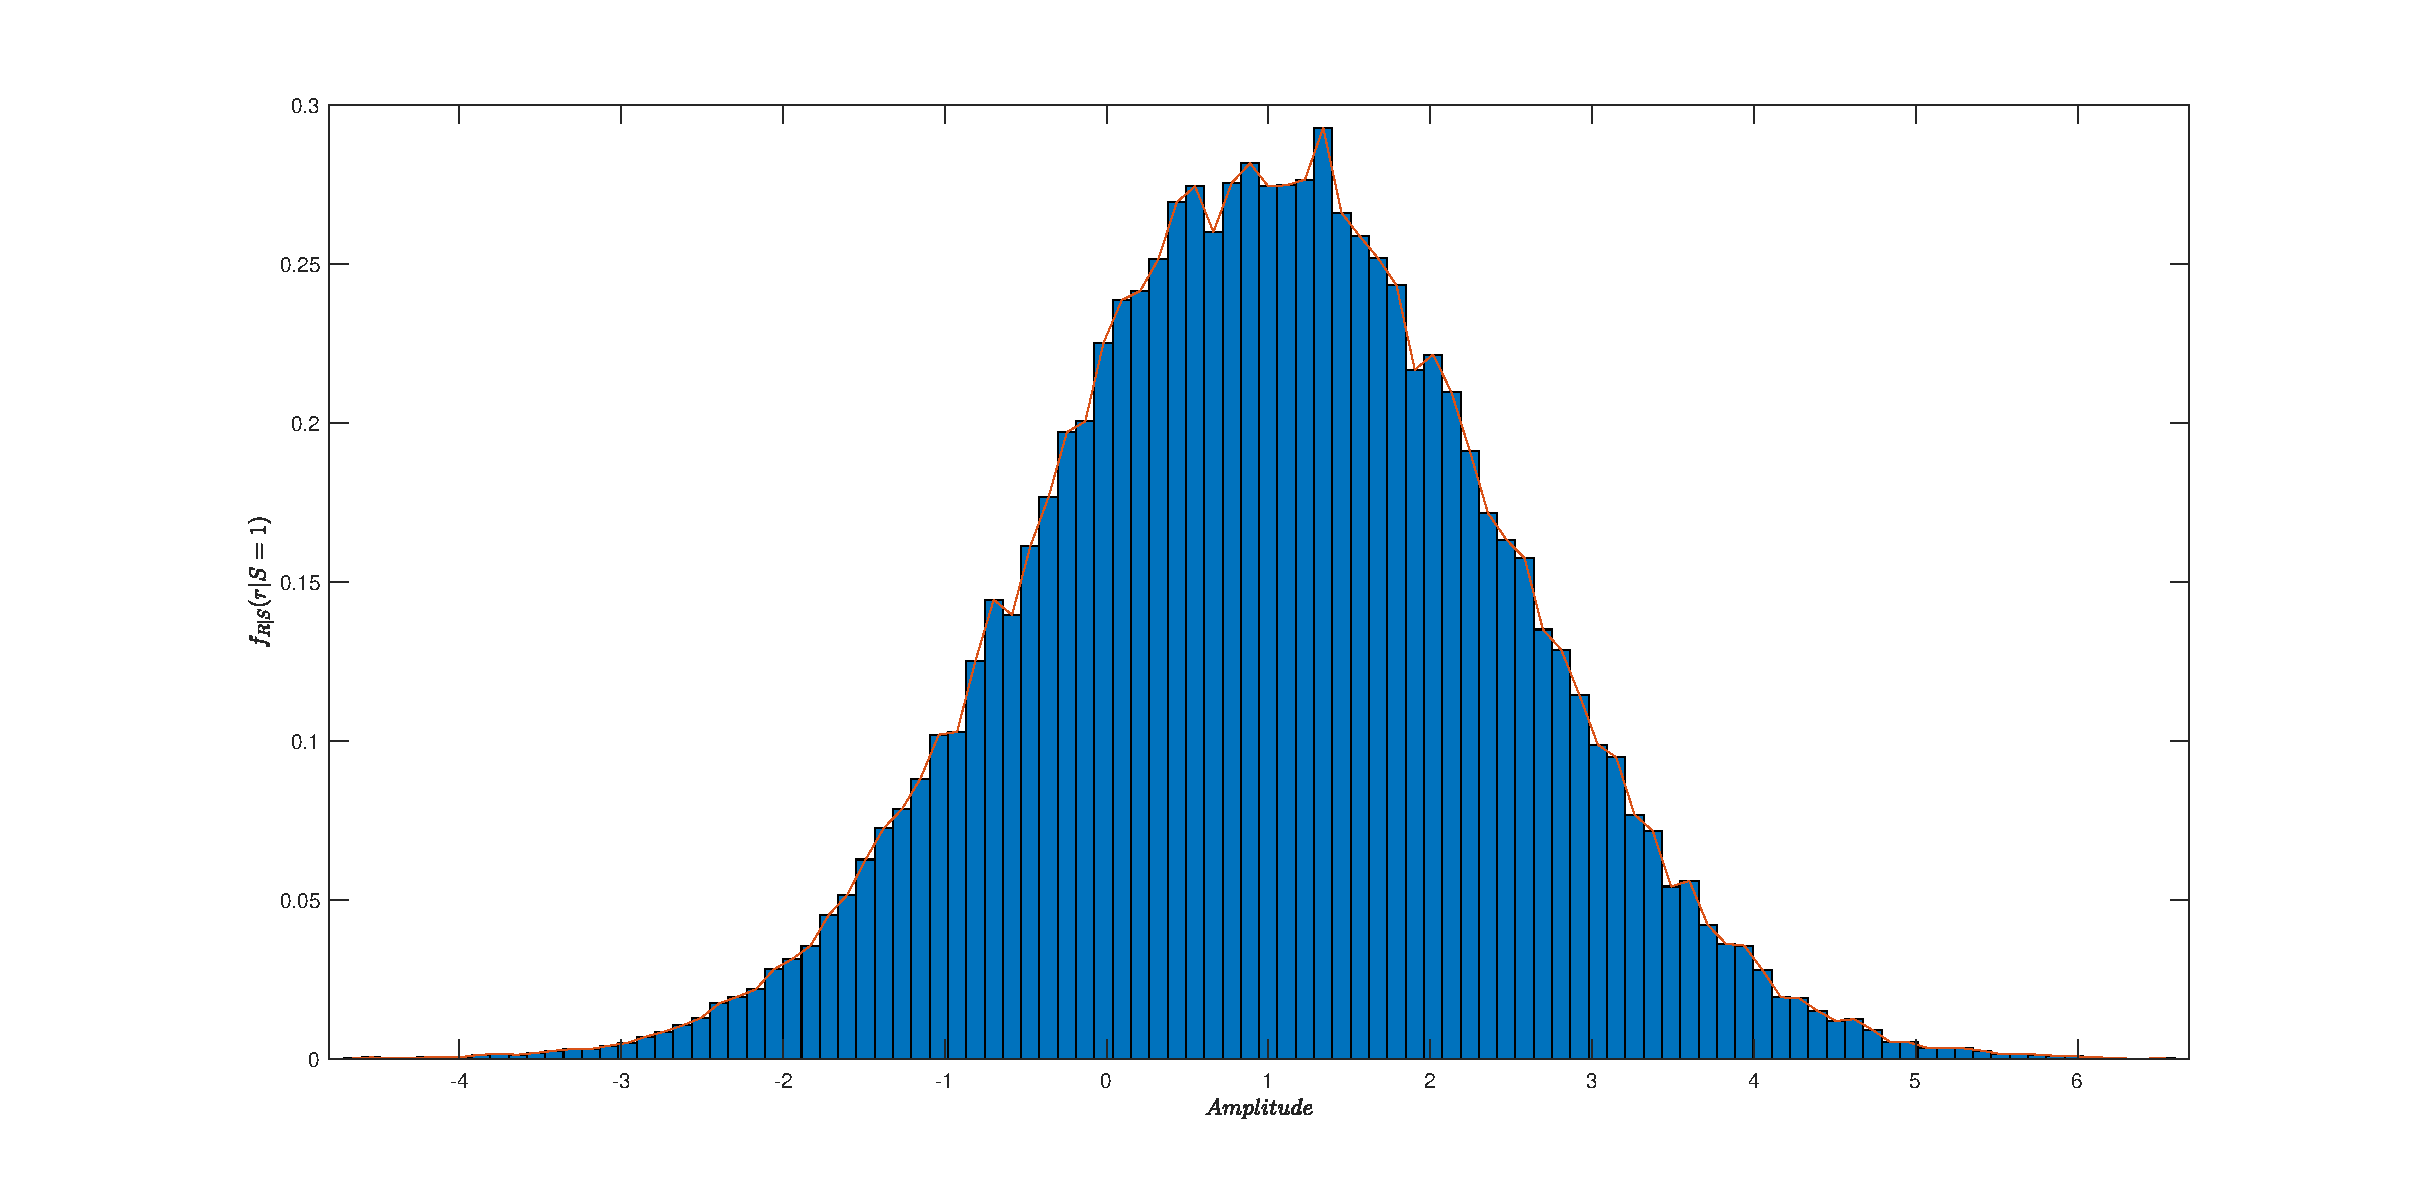
\includegraphics[scale=0.38]{figures/q6f1}
	\caption{$f_{R|S}(r|S=A)$ when interference is added}
\end{figure}

\begin{figure}[!h]
	\centering
	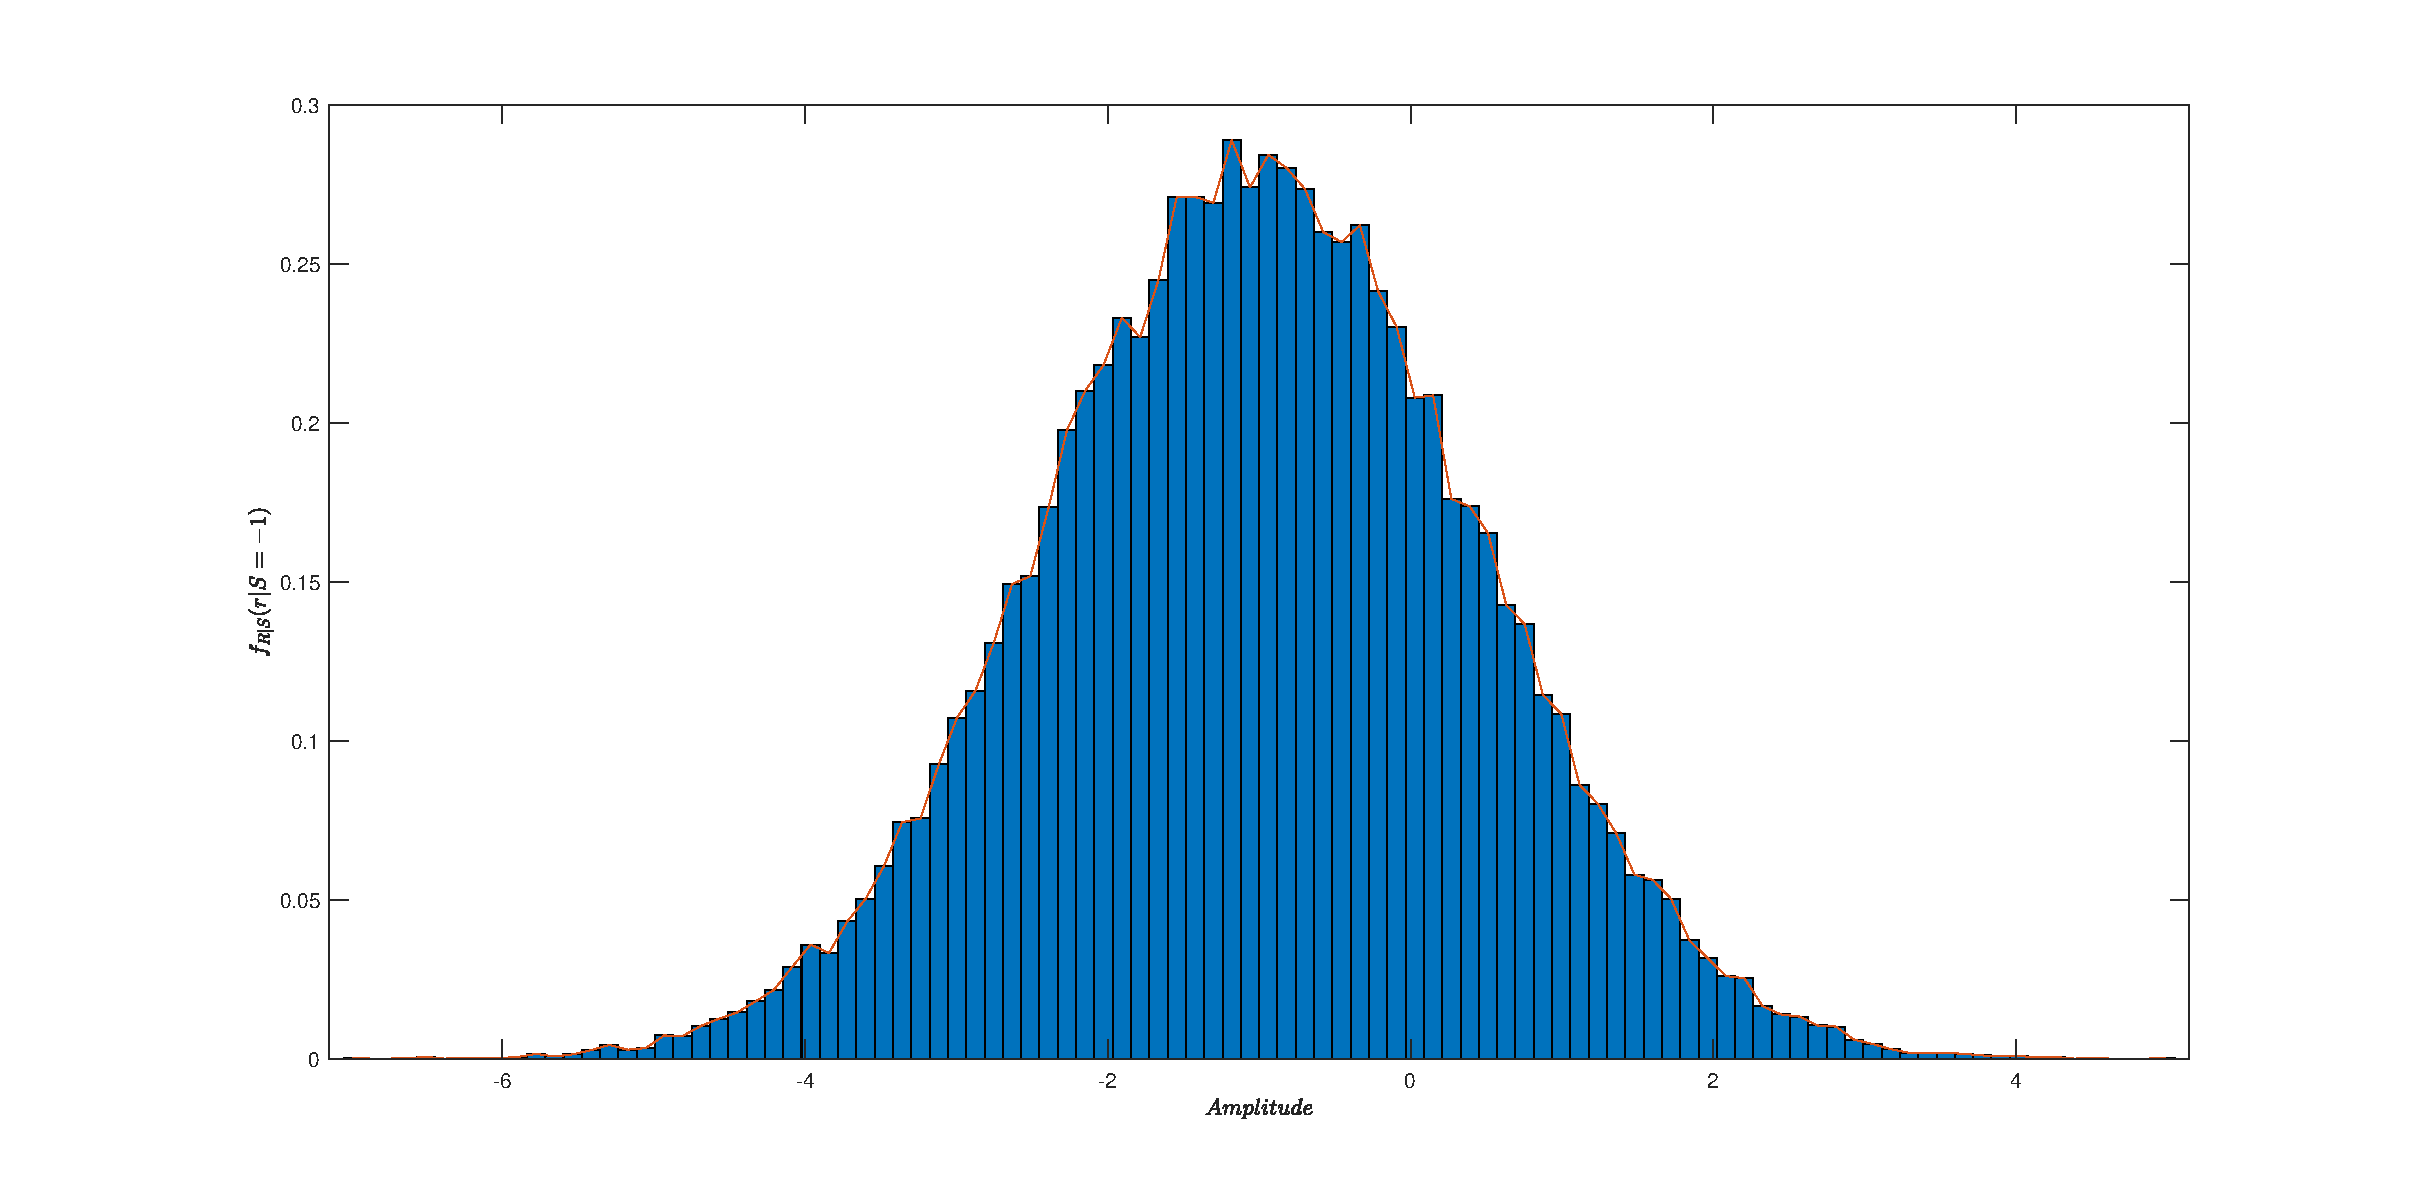
\includegraphics[scale=0.38]{figures/q6f2}
	\caption{$f_{R|S}(r|S= -A)$  when interference is added}
\end{figure}

\pagebreak
\subsection{Impact of A on the Conditional PDFs under additional interference}
\begin{figure}[!h]
	\centering
	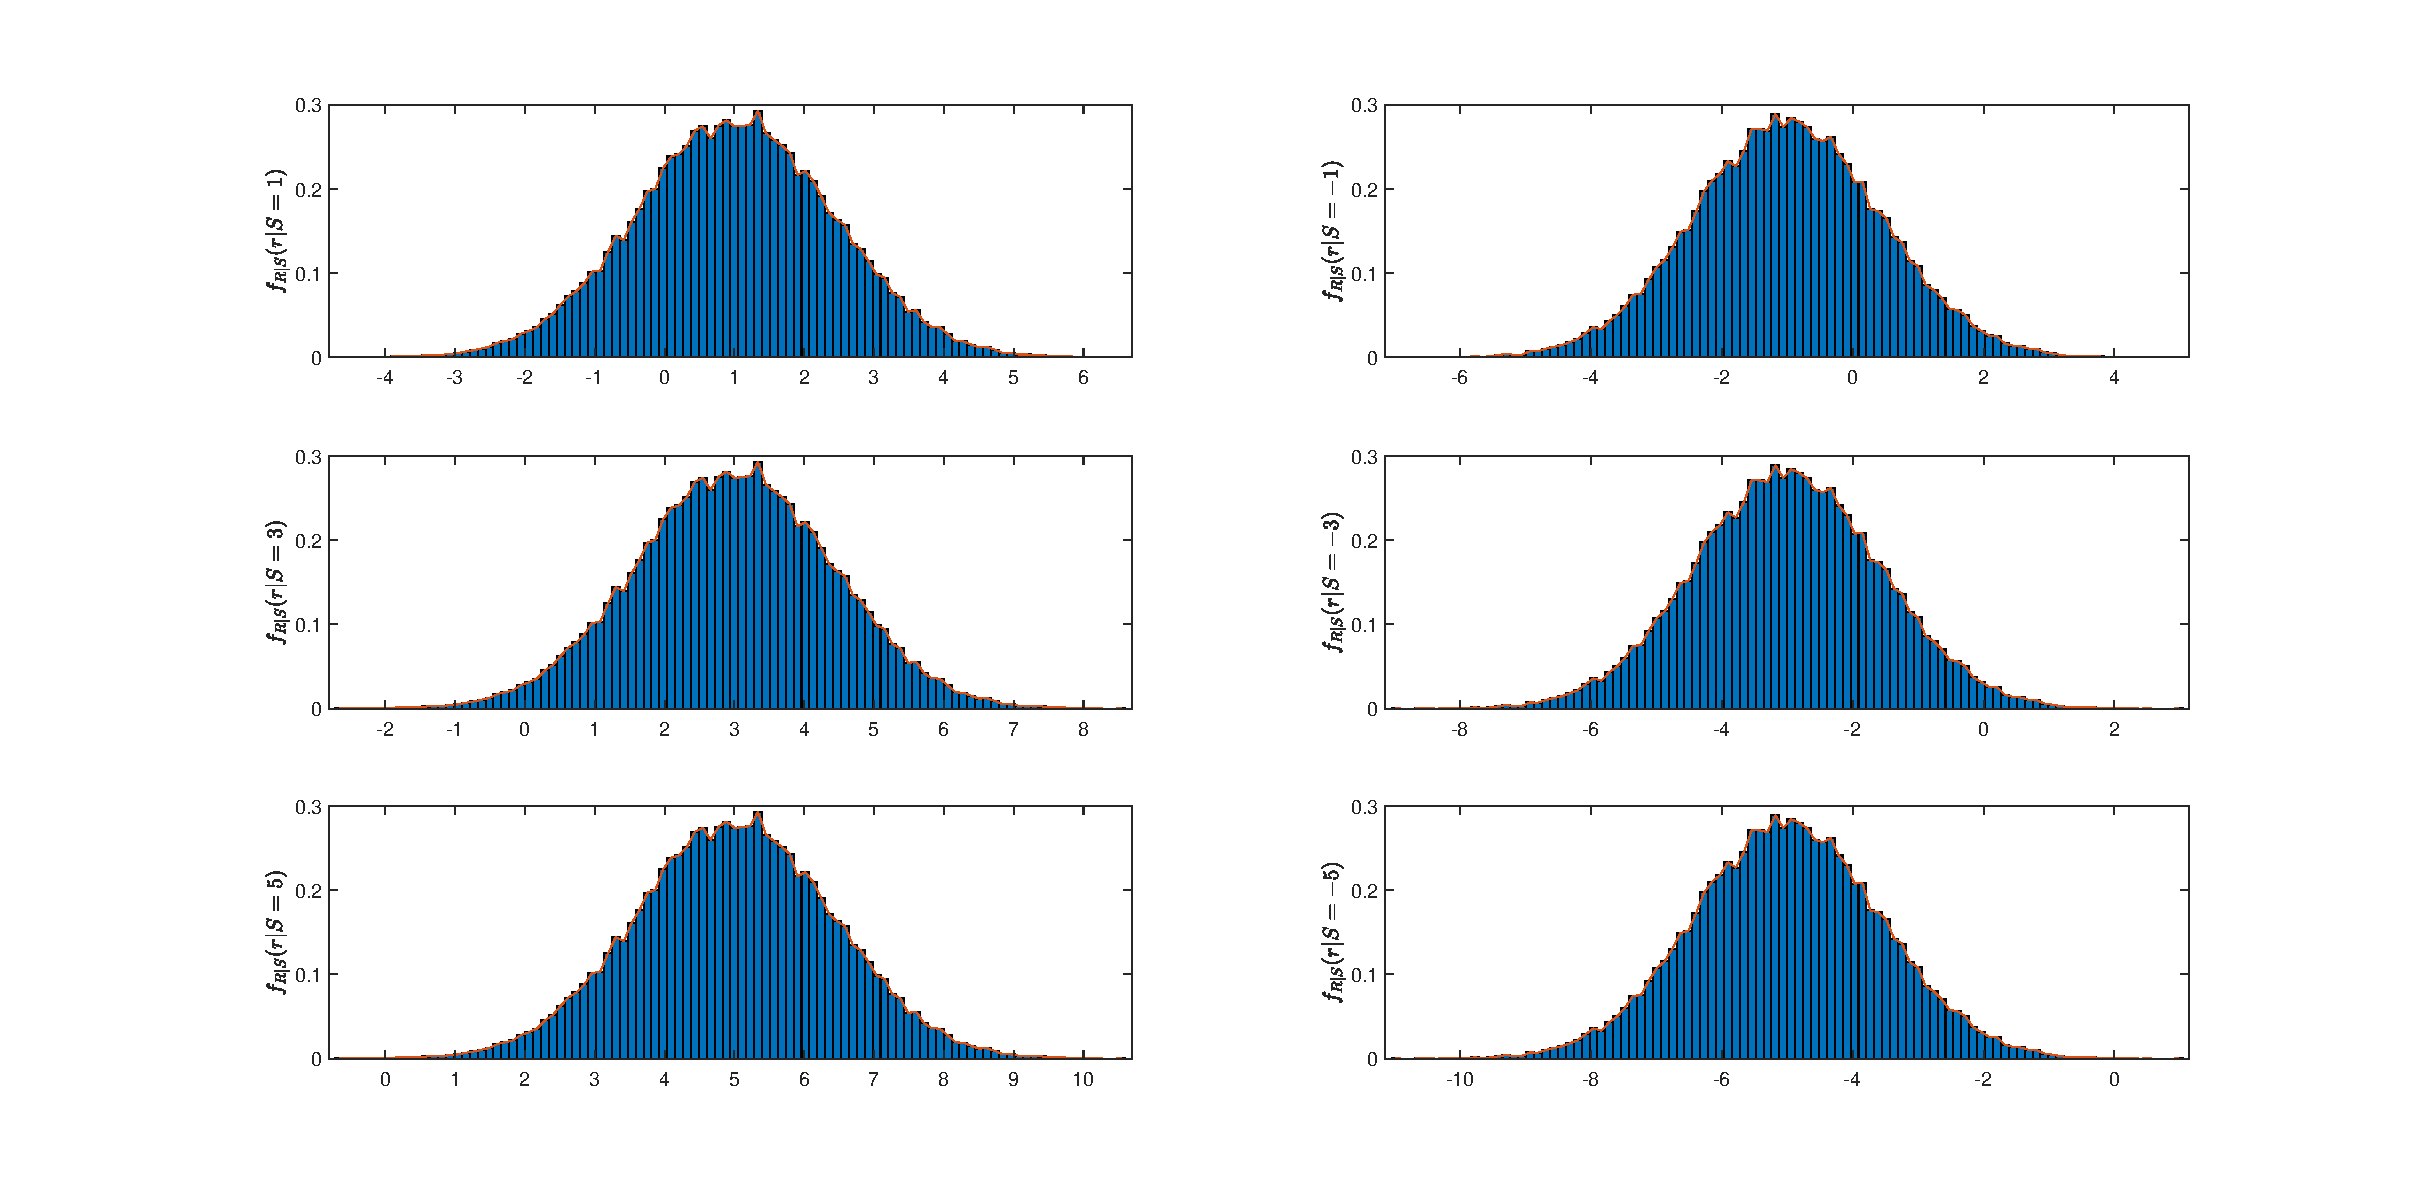
\includegraphics[scale=0.45]{figures/q6f3}
	\caption{Impact of A on the Conditional PDFs under additional interference}
\end{figure}

\subsection{Expected Values of the distributions and under additional interference}

As previously described interference affects only to the variance of the distribution. Therefore the Expected Values remains almost the same.\\

\begin{tabular}[!h]{l c r}
	Expected value $E[R]$& = & -0.0012806\\
	Expected value $E[R|S=A]$ &=& 0.99798\\
	Expected value $E[R|S=-A]$& =& -0.99949\\
	
\end{tabular}

\subsection{Marginal PDF of R $f_R(r)$ and under additional interference}
\begin{figure}[!h]
	\centering
	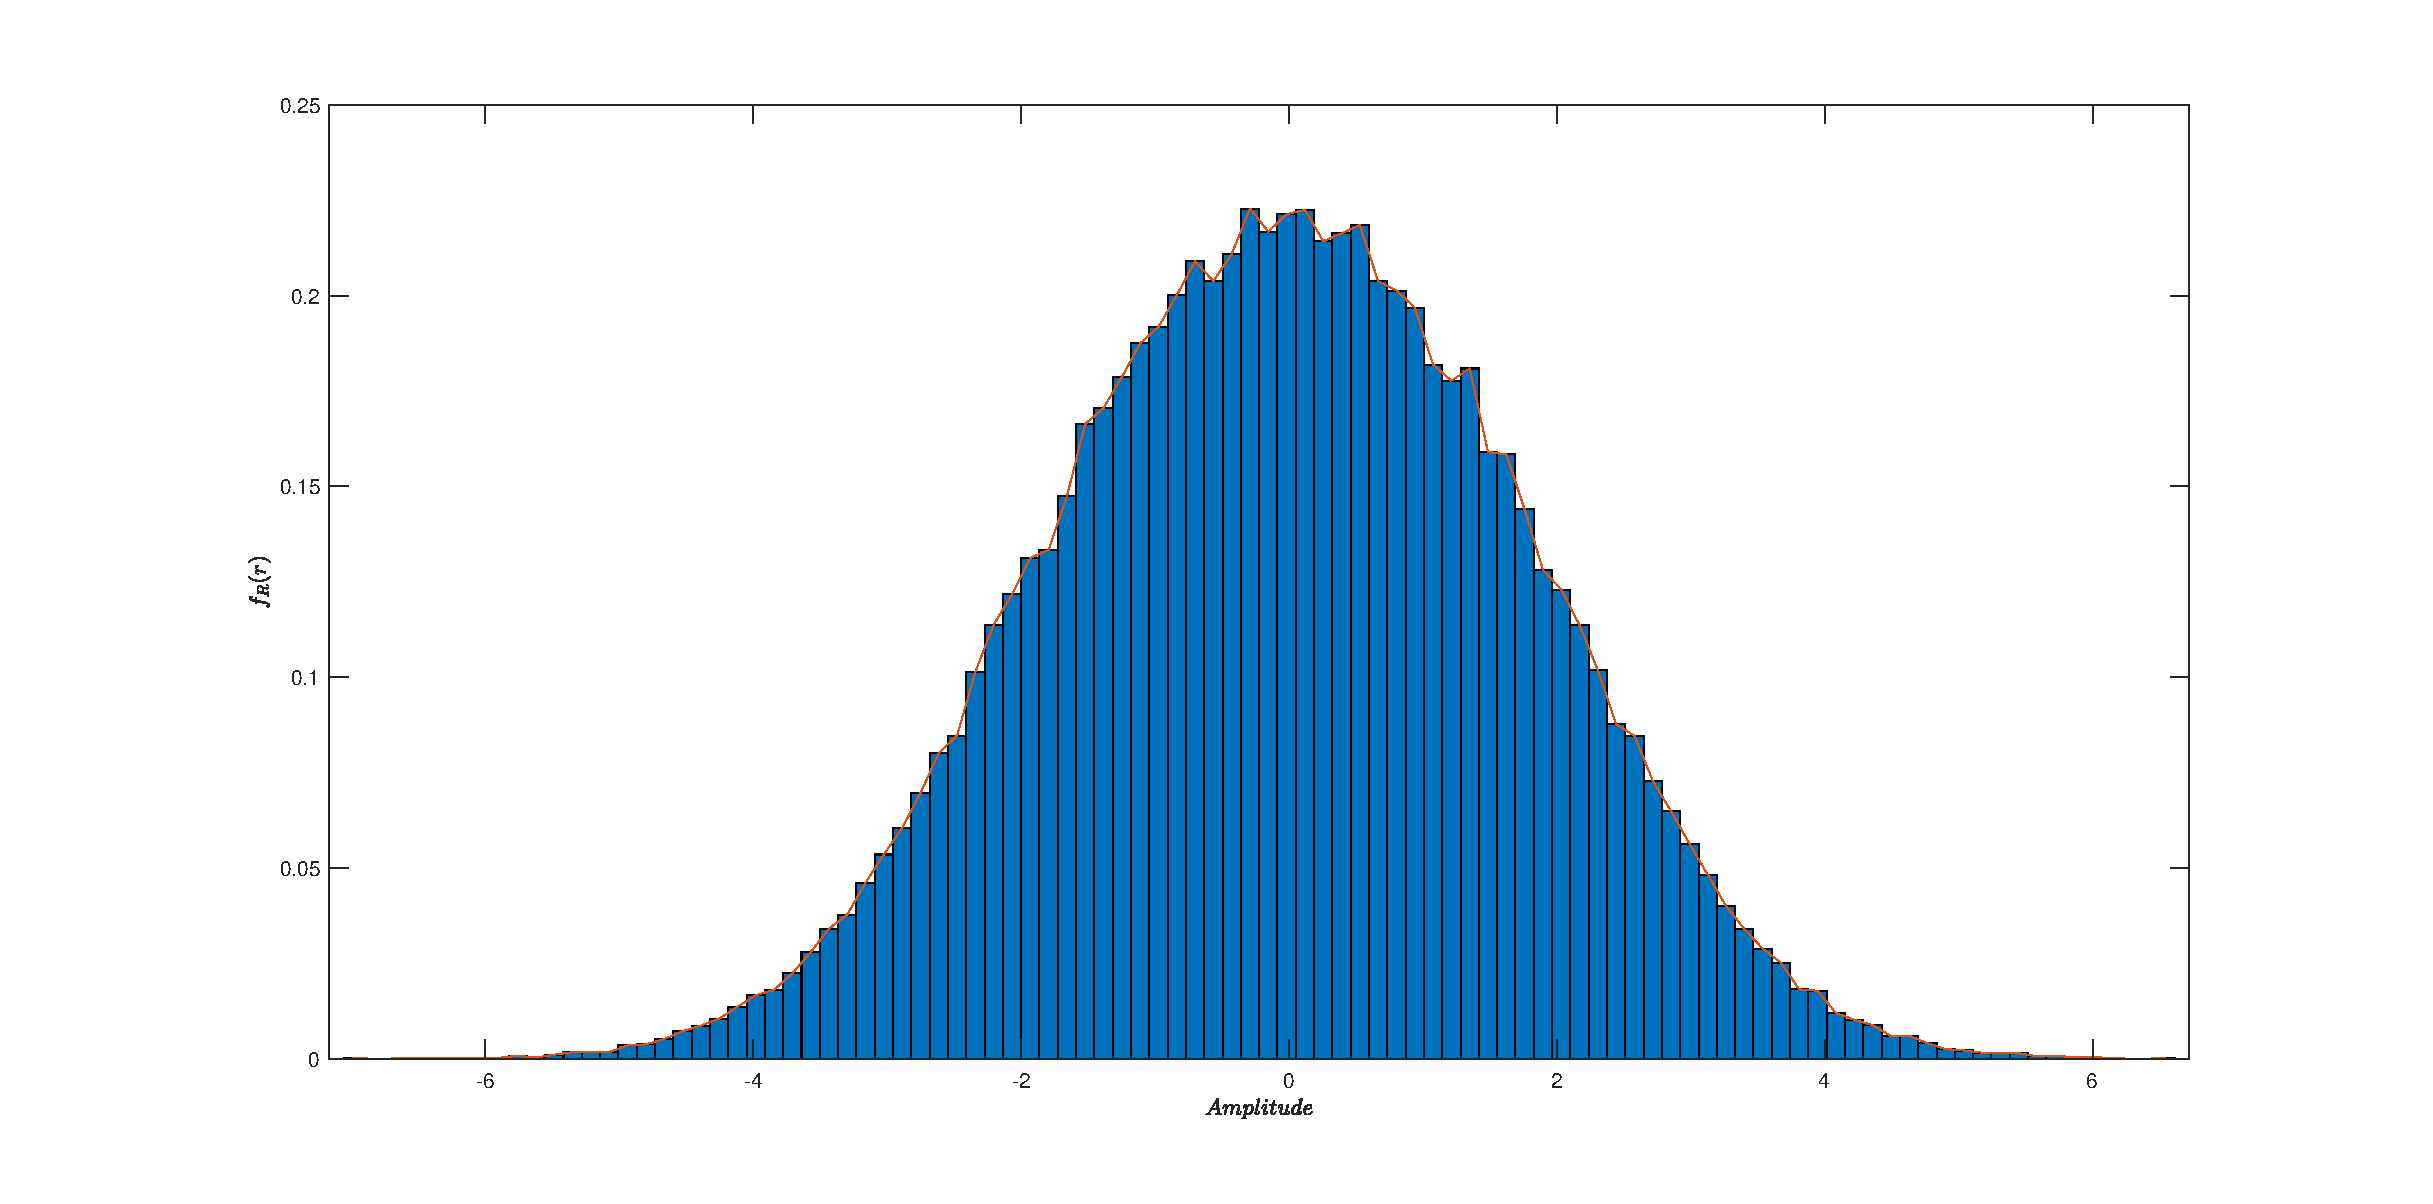
\includegraphics[scale=0.38]{figures/q6f4}
	\caption{Marginal PDF of R $f_R(r)$ under additional interference}
\end{figure}

\section{Question 7: Effect of Scaling when the number of bins = 100 and A = 1 and $\sigma^2 = 1$}

Effect of scaling of the pulse sequence(S), on the conditional probability distributions has the same effect as changing the signal level `A'. Therefore the figures and the subsections will be the same as that of Question 5.\\

Therefore only the behavior of Marginal distribution of R(received signal) is illustrated here. As it was not considered in earlier sections.

\begin{figure}[!h]
	\centering
	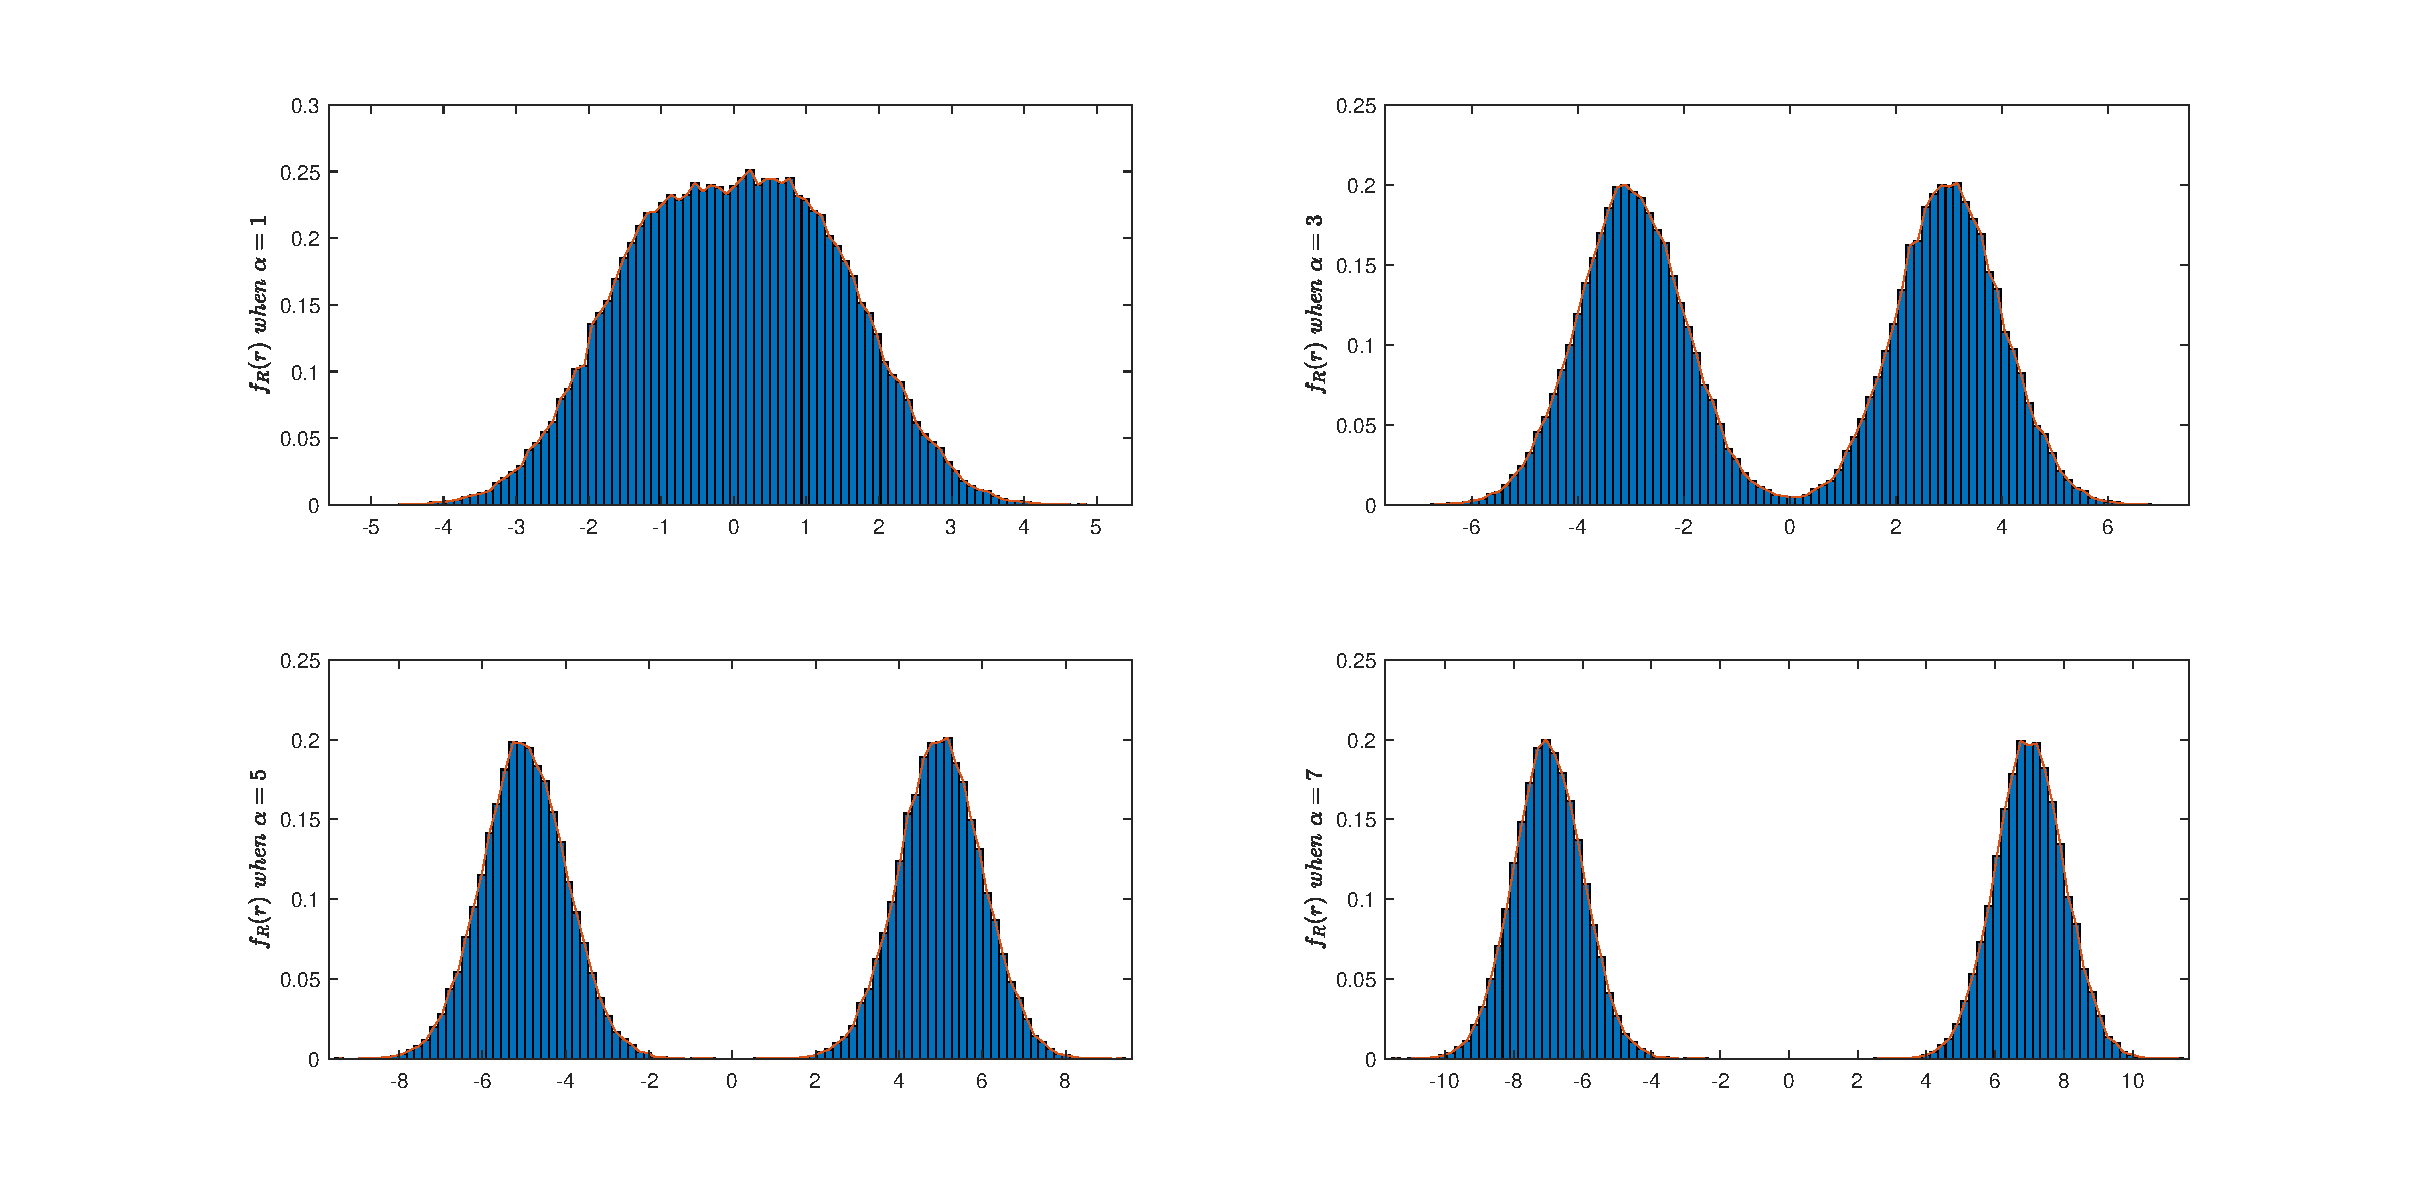
\includegraphics[scale=0.45]{figures/q7f1}
	\caption{Effect of Scaling on the Marginal PDF of R $f_R(r)$}
\end{figure}

The first sub-figure of the above figure shows the instance without any scaling. when the scale is increased, the distribution tends to divide in to two separate peaks centered around $+\alpha$ and $-\alpha$ as expected due to the lower variance than the scaling factor.

\begin{appendices}
	\section{Matlab Code for the Simulation}
	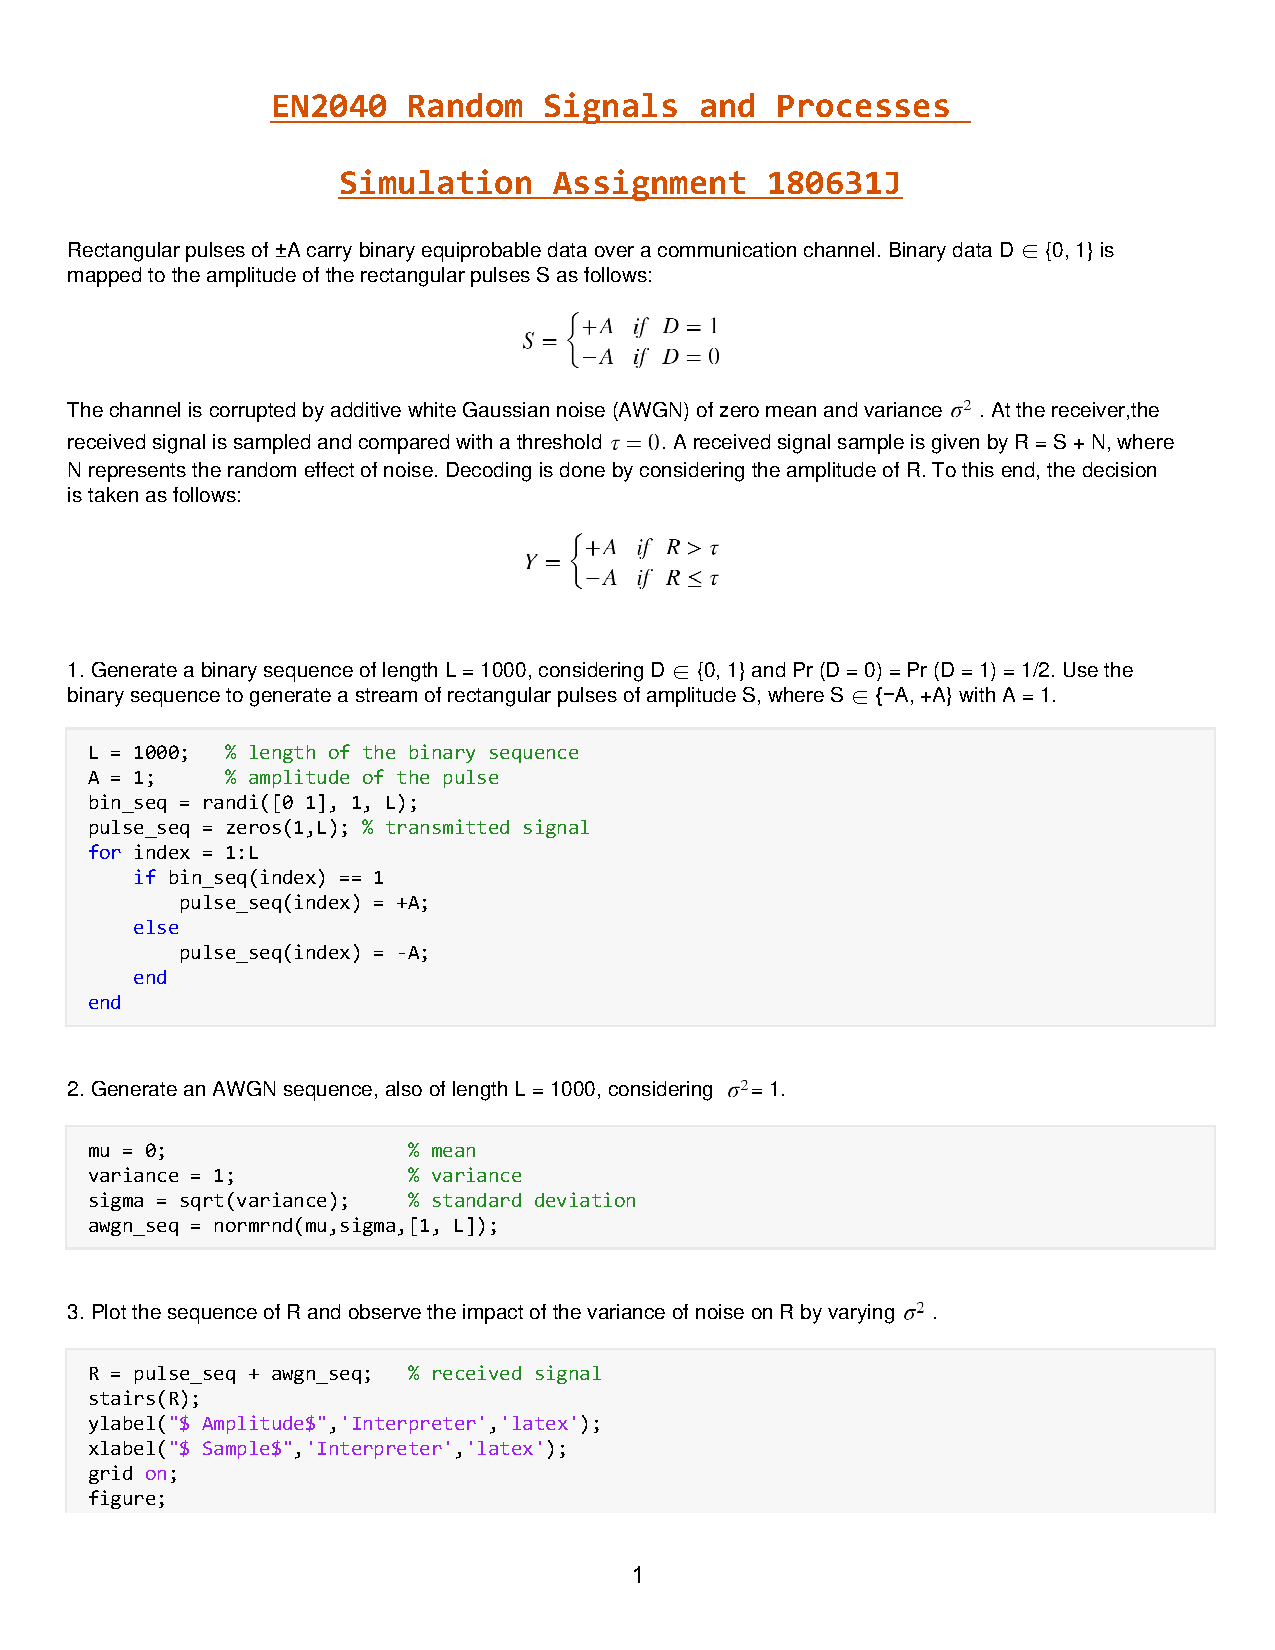
\includepdf[pages=-]{code/code.pdf}
\end{appendices}



%---------------------------------------------------------------------------
\end{document}
-
